\documentclass[a4paper,12pt]{extarticle}
\usepackage{geometry}
\usepackage[T2A,T1]{fontenc}
\usepackage[utf8]{inputenc}
\usepackage[english,russian]{babel}
\usepackage{csquotes}
\usepackage{amsmath}
\usepackage{amsthm}
\usepackage{amssymb}
\usepackage{fancyhdr}
\usepackage{setspace}
\usepackage{graphicx}
\usepackage{colortbl}
\usepackage{tikz}
\usepackage{pgf}
\usepackage{subcaption}
\usepackage{listings}
\usepackage{fancyvrb}
\usepackage{enumitem}
\usepackage{indentfirst}
\usepackage[colorlinks,linkcolor=blue,bookmarks=false,hypertexnames=true, urlcolor=blue]{hyperref} 
\usepackage{indentfirst}
\usepackage{mathtools}
\usepackage{booktabs}
\usepackage{array}
\usepackage{longtable}
\usepackage[flushleft]{threeparttable}
\usepackage{tablefootnote}
\newcolumntype{L}[1]{>{\raggedright\arraybackslash}p{#1}}
\emergencystretch=2em
\lstdefinestyle{jsonblock}{
	basicstyle=\ttfamily\footnotesize,
	breaklines=true,
	breakatwhitespace=false,
	frame=single,
	columns=fullflexible,
	keepspaces=true,
	showstringspaces=false,
	xleftmargin=0.3cm,
	xrightmargin=0.3cm
}
\DefineVerbatimEnvironment{jsonblock}{Verbatim}{fontsize=\footnotesize, frame=single, xleftmargin=0.3cm}
\newcommand{\tzsection}[1]{%
	\par\bigskip
	\phantomsection
	\addcontentsline{toc}{subsection}{#1}%
	\noindent{\large\bfseries #1}\par\nobreak\medskip
}
\newcommand{\tzsubsection}[1]{%
	\par\medskip
	\phantomsection
	\addcontentsline{toc}{subsubsection}{#1}%
	\noindent{\bfseries #1}\par\nobreak\smallskip
}
\newcommand{\tzpara}[1]{\medskip\noindent\textbf{#1}\par\nobreak\smallskip}
\newcommand{\tzmethod}[1]{%
	\medskip
	\noindent\colorbox{black!7}{%
		\parbox{\dimexpr\linewidth-2\fboxsep\relax}{\textbf{\texttt{#1}}}%
	}%
	\par\nobreak\smallskip
}
\newcommand{\tzlabel}[1]{\smallskip\noindent\emph{#1:}\par\nobreak\smallskip}
\newenvironment{tzcompact}{%
	\small
	\setlist[enumerate]{label=\arabic*., itemsep=0.15em, topsep=0.35em, parsep=0pt}
	\setlist[itemize]{itemsep=0.15em, topsep=0.35em, parsep=0pt}
	\setlist[description]{itemsep=0.2em, topsep=0.35em, parsep=0pt, leftmargin=3.9cm, style=nextline}
}{}

\usepackage{chngcntr} % нумерация графиков и таблиц по секциям
\counterwithin{table}{section}
\counterwithin{figure}{section}

\graphicspath{{graphics/}}%путь к рисункам

\makeatletter
\makeatother

\geometry{left=2.5cm}% левое поле
\geometry{right=1.0cm}% правое поле
\geometry{top=2.0cm}% верхнее поле
\geometry{bottom=2.0cm}% нижнее поле
\setlength{\parindent}{1.25cm}
\renewcommand{\baselinestretch}{1.5} % междустрочный интервал


\renewcommand{\theenumi}{\arabic{enumi}}% Меняем везде перечисления на цифра.цифра
\renewcommand{\labelenumi}{\arabic{enumi}}% Меняем везде перечисления на цифра.цифра
\renewcommand{\theenumii}{.\arabic{enumii}}% Меняем везде перечисления на цифра.цифра
\renewcommand{\labelenumii}{\arabic{enumi}.\arabic{enumii}.}% Меняем везде перечисления на цифра.цифра
\renewcommand{\theenumiii}{.\arabic{enumiii}}% Меняем везде перечисления на цифра.цифра
\renewcommand{\labelenumiii}{\arabic{enumi}.\arabic{enumii}.\arabic{enumiii}.}% Меняем везде перечисления на цифра.цифра

\begin{document}
\input{title_kr}
\newpage
\setcounter{page}{2}

{
	\hypersetup{linkcolor=black}
	\tableofcontents
}

\newpage

\section*{Аннотация}
В работе описана разработка backend-сервиса для трэвел-приложения, которое позволяет пользователям создавать городские маршруты, публиковать на их основе готовые впечатления, покупать их и проходить маршрут с фиксацией прогресса. Основной результат проекта - работающий прототип серверной части, реализованный на FastAPI с асинхронным доступом к базе данных через SQLAlchemy и PostgreSQL. Система включает регистрацию и авторизацию пользователей, разделение ролей, управление маршрутами и точками маршрута, модерацию, витрину впечатлений, покупки через pay-заглушку, отзывы, рекомендации, realtime-обновление прогресса, аналитику и BFF-методы для будущего frontend. Отдельное внимание уделено формальному API-контракту: все ответы возвращаются в едином формате, ошибки нормализованы, а основные пользовательские сценарии проверены автоматическими тестами.

\addcontentsline{toc}{section}{Аннотация}

% \pagebreak

\section{Введение}

Современные городские сервисы всё чаще ориентированы не только на поиск отдельных мест, но и на создание цельного пользовательского опыта: прогулки, экскурсии, тематического маршрута или самостоятельного путешествия. Для такого продукта недостаточно хранить список достопримечательностей. Требуется backend, который связывает маршруты, авторов, покупки, прохождение, отзывы, рекомендации и аналитику в единую систему.

Целью курсового проекта является разработка серверной части трэвел-приложения, в котором пользователь может создавать маршруты, превращать их в готовые впечатления, публиковать их в витрине, покупать опубликованные впечатления и проходить их с сопровождением по точкам маршрута. Задача является программным проектом: основной результат работы - не исследование алгоритма, а реализованный прототип системы с формализованным API, моделью данных, правилами доступа и проверками качества.

В ходе работы были сформулированы требования к продукту, выделены основные роли пользователей и домены системы, спроектирована структура REST API, реализованы серверные модули и автоматические проверки ключевых сценариев. Разработка велась по техническому заданию проекта. При реализации использованы FastAPI, SQLAlchemy, PostgreSQL и JWT-механизм авторизации.

\section{Анализ предметной области и постановка задачи}

\subsection{Предметная область}

Предметная область проекта - цифровые сервисы для городских прогулок и путешествий. Пользователь такого сервиса ожидает, что приложение не просто покажет набор мест на карте, а предложит законченное впечатление: маршрут с последовательностью точек, описанием, длительностью, ценой, отзывами и понятным процессом прохождения.

В рамках проекта были выделены следующие базовые сущности:
\begin{itemize}
	\item маршрут - последовательность точек, которую пользователь проходит в определённом порядке
	\item точка маршрута - географическая точка с координатами, описанием и порядковым номером
	\item впечатление - опубликованный пользовательский продукт, созданный на основе маршрута
	\item витрина - публичный каталог опубликованных впечатлений
	\item покупка - запись о приобретении впечатления пользователем
	\item прогресс - состояние прохождения впечатления пользователем
	\item аналитическое событие - запись о значимом действии пользователя или системы
\end{itemize}

Ключевая особенность предметной области состоит в том, что одна и та же сущность должна поддерживать разные состояния жизненного цикла. Например, маршрут может быть черновиком, находиться на модерации, быть опубликованным или архивированным. Поэтому backend должен не только выполнять CRUD-операции, но и контролировать допустимые переходы статусов, права доступа и связанность данных.

\subsection{Проблема и актуальность}

Обычный каталог мест плохо покрывает сценарий самостоятельной прогулки: пользователь вынужден сам выбирать порядок посещения точек, сверять расстояния, искать описания и понимать, завершил ли он маршрут. С другой стороны, авторам городских прогулок нужен инструмент публикации готовых впечатлений, а администраторам - механизм контроля качества и безопасности контента.

Практическая ценность проекта заключается в создании backend-основы, на которую можно подключить мобильный или web-клиент. Такая серверная часть берёт на себя хранение данных, правила доступа, публикацию контента, оплату через заглушку, realtime-прогресс и сбор аналитики. Это снижает сложность будущего frontend и позволяет развивать продукт по доменам.

\subsection{Постановка задачи}

Необходимо разработать backend-сервис, который предоставляет API для следующих групп пользователей:
\begin{itemize}
	\item обычный пользователь регистрируется, просматривает витрину, покупает и проходит впечатления, оставляет отзывы
	\item автор создаёт маршруты и впечатления, а после верификации публикует их без предварительной модерации
	\item администратор модерирует маршруты и впечатления, блокирует пользователей, назначает роль автора и просматривает аналитику
\end{itemize}

Сервис должен обеспечивать единый формат ответов, проверку входных данных, авторизацию по JWT, хранение данных в реляционной базе, realtime-обновление прогресса через WebSocket и набор автоматических тестов для основных сценариев.

\newpage

\section{Техническое задание}

\begingroup
\begin{tzcompact}
\begin{sloppypar}
\tzsection{1. Назначение продукта}

Разрабатывается backend-сервис для трэвел-приложения, которое помогает пользователю получать новые впечатления во время поездок, прогулок и путешествий по городу.

\tzsubsection{1.1. Термины и определения}

В рамках данного ТЗ используются следующие определения:

\begin{description}
\item[\texttt{маршрут}]
последовательность точек, которые предлагаются пользователю пройти в определённом порядке
\item[\texttt{точка маршрута}]
отдельная географическая точка внутри маршрута с координатами, \\описанием и порядком прохождения
\item[\texttt{впечатление}]
готовый пользовательский продукт, построенный на основе маршрута и \\подготовленный для показа в витрине, покупки и прохождения
\item[\texttt{витрина}]
каталог опубликованных впечатлений, доступных для просмотра, \\фильтрации, выбора и покупки
\item[\texttt{верифицированный пользователь}]
пользователь, прошедший проверку и получивший роль \path|author|
\item[\texttt{профиль пользователя}]
набор пользовательских данных, который хранится в системе и возвращается после авторизации
\item[\texttt{покупка}]
запись о том, что пользователь инициировал или успешно завершил \\приобретение впечатления
\item[\texttt{прогресс}]
текущее состояние прохождения впечатления пользователем
\item[\texttt{рекомендации}]
список впечатлений, подобранных системой по правилам, указанным \\в разделе \path|6.8|
\item[\texttt{аналитическое событие}]
запись о действиях пользователя или системы, события указаны \\в разделе \path|6.10|
\item[\path|BFF|]
набор API-методов, которые собирают данные из нескольких частей backend и возвращают их в форме, удобной для frontend
\end{description}

Продукт должен решать следующие задачи:

\begin{enumerate}
\item пользователь должен иметь возможность создавать маршруты
\item пользователь должен иметь возможность превращать маршрут в готовое впечатление
\item пользователь должен иметь возможность просматривать витрину опубликованных впечатлений
\item пользователь должен иметь возможность покупать впечатления
\item пользователь должен иметь возможность проходить впечатление с сопровождением по маршруту
\item система должна формировать рекомендации
\item система должна фиксировать основные пользовательские действия
\end{enumerate}

\tzsection{2. Сценарии использования}

\tzsubsection{2.1. Основной пользовательский сценарий}

\begin{enumerate}
\item пользователь регистрируется и входит в систему
\item пользователь открывает витрину впечатлений
\item пользователь просматривает карточку впечатления
\item пользователь покупает впечатление (впечатление необязательно платное, оно может быть и бесплатным)
\item пользователь запускает прохождение впечатления
\item клиент передаёт координаты пользователя
\item система определяет прогресс прохождения маршрута
\item пользователь завершает прохождение
\item в течение прохождения этапов система фиксирует события аналитики
\end{enumerate}

\tzsubsection{2.2. Сценарий автора}

\begin{enumerate}
\item автор создаёт маршрут
\item автор добавляет точки маршрута
\item автор отправляет маршрут на публикацию
\item маршрут автора публикуется сразу после отправки
\item автор создаёт впечатление на основе маршрута
\item автор отправляет впечатление на публикацию
\item впечатление автора публикуется сразу после отправки
\item впечатление автора сразу появляется в витрине
\end{enumerate}

\tzsubsection{2.3. Сценарии администратора}

\begin{enumerate}
\item администратор просматривает маршруты и впечатления пользователей в статусе \path|on_moderation|
\item администратор публикует или отклоняет маршруты и впечатления неверифицированных пользователей
\item администратор блокирует или разблокирует пользователя
\item администратор переводит пользователя в статус верифицированного автора
\item администратор имеет доступ к аналитическим данным
\end{enumerate}

\tzsection{3. Границы проекта}

\tzsubsection{3.1. Входит в проект}

\begin{enumerate}
\item регистрация и авторизация пользователей
\item разделение прав ролей \path|user|, \path|author|, \path|admin| (права на каждый API-метод описаны в 7.3)
\item управление маршрутами
\item управление точками маршрута
\item создание и редактирование впечатлений
\item модерация маршрутов и впечатлений
\item витрина впечатлений
\item покупка впечатлений через pay-заглушку
\item отзывы и оценки
\item рекомендации без ML
\item отслеживание прогресса маршрута в реальном времени
\item аналитика действий пользователя
\item BFF API-методы для будущего frontend
\item проксирование внешних API, таких как картографических
\end{enumerate}

\tzsubsection{3.2. Не входит в проект}

\begin{enumerate}
\item реальные платёжные системы
\item офлайн-навигация
\item ML-рекомендации
\item социальная сеть
\item сложная мультимедийная платформа
\end{enumerate}

\tzsection{4. Роли и правила доступа}

\tzsubsection{4.1. Роли}

\begin{enumerate}
\item \path|user|:
просматривает витрину, покупает и проходит впечатления, оставляет отзывы, создаёт маршруты и впечатления, которые публикуются только после модерации
\item \path|author|:
является верифицированным пользователем и имеет все возможности \path|user|, но его маршруты и впечатления публикуются сразу без предварительной модерации
\item \path|admin|:
имеет все возможности \path|author|, а также выполняет модерацию, блокировку пользователей и просмотр аналитики
\end{enumerate}

\tzsubsection{4.2. Общие правила доступа}

\begin{enumerate}
\item публичные API-методы не требуют авторизации
\item защищённые API-методы требуют валидного JWT (неистёкшего по времени)
\item изменение сущности разрешено только владельцу сущности либо \path|admin|
\item административные API-методы доступны только \path|admin|
\item пользователь не должен получать доступ к чужим покупкам, прогрессу и черновикам
\item в витрине показываются только впечатления в статусе \path|published|
\item маршруты и впечатления пользователя с ролью \path|user| должны проходить модерацию перед публикацией
\item маршруты и впечатления пользователя с ролью \path|author| публикуются сразу
\item WebSocket-подключение должно быть доступно только авторизованному пользователю
\item заблокированный пользователь не должен иметь доступ к защищённым API-методам даже при наличии валидного JWT
\end{enumerate}

\tzsection{5. Общие требования к данным}

\tzsubsection{5.1. Общие правила валидации}

\begin{enumerate}
\item все входные данные должны проходить серверную валидацию до выполнения бизнес-логики (пункты 5.1 и 7.2)
\item все строковые поля должны обрезаться по краям от лишних пробелов перед сохранением
\item пустые строки не должны приниматься как валидные значения обязательных полей
\item идентификаторы должны передаваться как положительные целые числа
\item даты и время должны передаваться и возвращаться в ISO 8601 (\path|YYYY-MM-DDThh:mm:ss|)
\item ошибки валидации должны возвращаться в предсказуемом формате (пункт 7.1)
\end{enumerate}

\tzsubsection{5.2. Общие правила для текстовых полей}

\begin{enumerate}
\item названия маршрутов, впечатлений и точек должны содержать от \path|3| до \path|120| символов
\item описания маршрутов и впечатлений должны содержать от \path|10| до \path|2000| символов
\item комментарий в отзыве должен содержать от \path|1| до \path|1000| символов
\item текстовые поля должны допускать буквы кириллицы и латиницы, цифры, пробел, а также базовые знаки пунктуации
\item управляющие символы и пустые значения должны отклоняться
\end{enumerate}

\tzsubsection{5.2.1. Термины удаления}

В рамках ТЗ используются следующие трактовки удаления:

\begin{enumerate}
\item \texttt{удаление}:
пользовательский сценарий удаления сущности из интерфейса или API
\item \texttt{физическое удаление}:
техническая операция, при которой запись удаляется из базы данных без сохранения
\item \texttt{архивирование}:
мягкое удаление, при котором запись сохраняется в базе данных и переводится в статус \path|archived|
\end{enumerate}

\tzsubsection{5.3. Связи сущностей}

В системе фиксируются следующие основные связи между сущностями:

\begin{enumerate}
\item \path|User 1:N Route|
\item \path|Route 1:N RoutePoint|
\item \path|Route 1:N Impression|
\item \path|User 1:N Purchase|
\item \path|Impression 1:N Review|
\item \path|User 1:N Review|
\item \path|User 1:N AnalyticsEvent|
\item \path|User 1:N Progress|
\end{enumerate}

\tzsection{6. Функциональные требования по доменам}

В рамках данного ТЗ доменом называется функциональная область системы, объединяющая близкие пользовательские сценарии, сущности и связанные с ними API-методы. Например, сценарии создания маршрута, редактирования маршрута и отправки маршрута на публикацию относятся к домену маршрутов.

\tzsubsection{6.1. Пользователи и профиль}

\tzpara{6.1.1. Определение профиля}

Профиль пользователя в рамках системы представляет собой совокупность пользовательских данных, которые backend хранит и возвращает после авторизации. Профиль не создаётся отдельным API-методом после регистрации, а возникает как результат регистрации пользователя.

\tzpara{6.1.2. Состав данных пользователя}

Пользователь должен содержать следующие поля:

\begin{enumerate}
\item \path|id|
\item \path|username|
\item \path|email|
\item \path|password_hash|
\item \path|role|
\item \path|is_blocked|
\item \path|created_at|
\item \path|updated_at|
\end{enumerate}

\tzpara{6.1.3. Пример JSON профиля}

\begin{jsonblock}
{
    "id": 1,
    "username": "for_example123",
    "email": "user@example.com",
    "role": "user",
    "is_blocked": false,
    "created_at": "2026-04-08T10:00:00Z",
    "updated_at": "2026-04-08T10:00:00Z"
}
\end{jsonblock}

\tzpara{6.1.4. Правила валидации}

\begin{enumerate}
\item \path|username| обязателен
\item \path|username| должен быть уникальным
\item \path|username| должен содержать от \path|3| до \path|30| символов
\item \path|username| должен содержать только латинские буквы, цифры и символ подчёркивания \path|_|
\item \path|email| обязателен и должен соответствовать формату email (базовая валидация email)
\item \path|email| должен быть уникальным
\item \path|password| обязателен
\item длина \path|password| должна быть от \path|8| до \path|64| символов
\item \path|password| должен содержать хотя бы одну букву, хотя бы одну цифру и хотя бы один специальный символ
\item \path|role| должен принадлежать одному из значений: \path|user|, \path|author|, \path|admin|
\item при публичной регистрации пользователю назначается роль \path|user|
\item роль \path|author| назначается только после верификации администратором
\item пароль должен храниться только в виде безопасного криптографического хэша
\end{enumerate}

\tzpara{6.1.5. Функциональные требования}

\begin{enumerate}
\item система должна обеспечивать регистрацию пользователя
\item система должна обеспечивать авторизацию пользователя
\item система должна обеспечивать получение профиля текущего пользователя
\item система должна обеспечивать блокировку и разблокировку пользователя администратором
\item система должна обеспечивать перевод пользователя в роль \path|author| после верификации администратором
\end{enumerate}

\tzpara{6.1.6. API-методы домена}

\tzmethod{POST /auth/register}

\tzlabel{Вход}

\begin{enumerate}
\item \path|username|
\item \path|email|
\item \path|password|
\end{enumerate}

\tzlabel{Что происходит}

\begin{enumerate}
\item проверяется уникальность username
\item проверяется уникальность email 
\item валидируется пароль 
\item пароль хэшируется
\item создаётся пользователь
\item пользователю назначается роль \path|user|
\item возвращается созданный профиль пользователя
\end{enumerate}

\tzlabel{Выход}

\begin{enumerate}
\item \path|access_token|
\item тип токена
\item идентификатор пользователя
\item username
\item email
\item роль
\end{enumerate}

\tzmethod{POST /auth/login}

\tzlabel{Вход}

\begin{enumerate}
\item \path|email| или \path|username|
\item \path|password|
\end{enumerate}

\tzlabel{Что происходит}

\begin{enumerate}
\item система проверяет существование пользователя
\item система сравнивает пароль с хэшем
\item при успехе выдаётся JWT
\end{enumerate}

\tzlabel{Выход}

\begin{enumerate}
\item \path|access_token|
\item тип токена
\item идентификатор пользователя
\item username
\item email
\item роль
\end{enumerate}

\tzmethod{GET /users/me}

\tzlabel{Вход}

\begin{enumerate}
\item JWT текущего пользователя
\end{enumerate}

\tzlabel{Что происходит}

\begin{enumerate}
\item система определяет пользователя по токену
\item возвращает профиль текущего пользователя
\end{enumerate}

\tzlabel{Выход}

\begin{enumerate}
\item JSON профиля пользователя (пункт 6.1.3)
\end{enumerate}

\tzmethod{PATCH /admin/users/\{user\_id\}/block}

\tzlabel{Вход}

\begin{enumerate}
\item идентификатор пользователя
\item флаг блокировки
\item JWT администратора
\end{enumerate}

\tzlabel{Что происходит}

\begin{enumerate}
\item проверяется роль \path|admin|
\item обновляется признак блокировки пользователя
\end{enumerate}

\tzlabel{Выход}

\begin{enumerate}
\item обновлённый профиль пользователя
\end{enumerate}

\tzmethod{PATCH /admin/users/\{user\_id\}/verify-author}

\tzlabel{Вход}

\begin{enumerate}
\item идентификатор пользователя
\item JWT администратора
\end{enumerate}

\tzlabel{Что происходит}

\begin{enumerate}
\item проверяется роль \path|admin|
\item пользователю назначается роль \path|author|
\end{enumerate}

\tzlabel{Выход}

\begin{enumerate}
\item обновлённый профиль пользователя
\end{enumerate}

\tzsubsection{6.2. Маршруты}

\tzpara{6.2.1. Назначение}

Маршрут представляет собой последовательность точек, которые пользователь должен пройти в определённом порядке. Маршрут является основой для создания впечатления.

\tzpara{6.2.2. Состав данных маршрута}

Маршрут должен содержать следующие поля:

\begin{enumerate}
\item \path|id|
\item \path|user_id|
\item \path|name|
\item \path|description|
\item \path|cities|
\item \path|duration_minutes|
\item \path|status|
\item \path|moderation_comment|
\item \path|created_at|
\item \path|updated_at|
\end{enumerate}

\tzpara{6.2.3. Источник данных для городов}

Поле \path|cities| должно заполняться пользователем при создании или редактировании маршрута.

Для работы с городами действуют следующие правила:

\begin{enumerate}
\item пользователь выбирает города из справочника одного выбранного картографического провайдера
\item backend использует \path|external_city_id| этого провайдера как основной идентификатор города
\item для каждого города backend сохраняет как минимум \path|external_city_id| и \path|name|
\item backend проверяет, что переданный город действительно существует в используемом справочнике провайдера
\item для одного маршрута не должны сохраняться дублирующиеся города с одинаковым \path|external_city_id|
\end{enumerate}

\tzpara{6.2.4. Пример JSON маршрута}

\begin{jsonblock}
{
    "id": 10,
    "user_id": 3,
    "name": "Прогулка по центру Москвы",
    "description": "Маршрут на два часа по основным точкам центра",
    "cities": [
      {
        "external_city_id": "12345",
        "name": "Москва"
      }
    ],
    "duration_minutes": 120,
    "status": "published",
    "moderation_comment": null,
    "created_at": "2026-04-08T10:00:00Z",
    "updated_at": "2026-04-08T10:00:00Z"
}
\end{jsonblock}

\tzpara{6.2.5. Статусы маршрута}

Маршрут должен поддерживать следующие статусы:

\begin{enumerate}
\item \path|draft|
\item \path|on_moderation|
\item \path|published|
\item \path|rejected|
\item \path|archived|
\end{enumerate}

Статус \path|draft| означает, что пользователь ещё редактирует маршрут и не отправил его на публикацию. Пока маршрут находится в \path|draft|, он не попадает на модерацию и не может быть показан в публичных списках.

\tzpara{6.2.5.1. Разрешённые переходы статуса}

Для маршрута должны поддерживаться следующие переходы:

\begin{enumerate}
\item \path|draft -> on_moderation| после \path|submit|, если владелец имеет роль \path|user|
\item \path|draft -> published| после \path|submit|, если владелец имеет роль \path|author|
\item \path|on_moderation -> published| по решению \path|admin|
\item \path|on_moderation -> rejected| по решению \path|admin|
\item \path|rejected -> draft| после доработки владельцем
\item \path|published -> archived| по решению владельца или \path|admin|
\end{enumerate}

При редактировании маршрута в статусе \path|published| маршрут должен переводиться обратно в \path|draft|.

\tzpara{6.2.6. Правила валидации}

\begin{enumerate}
\item \path|name| обязателен
\item \path|name| должен содержать от \path|3| до \path|120| символов
\item \path|description| обязателен
\item \path|description| должен содержать от \path|10| до \path|2000| символов
\item \path|cities| должен быть непустым массивом объектов города
\item в массиве \path|cities| должно быть от \path|1| до \path|10| значений
\item каждый объект города должен содержать \path|external_city_id| и \path|name|
\item \path|external_city_id| должен быть непустой строкой
\item \path|name| должен содержать от \path|2| до \path|80| символов
\item значения в \path|cities| должны храниться без дубликатов по \path|external_city_id|
\item отображаемое поле \path|name| должно нормализоваться по пробелам
\item \path|duration_minutes| должно быть целым числом от \path|1| до \path|1440|
\item \path|status| должен принадлежать фиксированному набору значений
\item \path|moderation_comment| может быть пустым, но при отклонении маршрута должен содержать от \path|1| до \path|1000| символов
\end{enumerate}

\tzpara{6.2.7. Функциональные требования}

\begin{enumerate}
\item система должна обеспечивать создание маршрута
\item система должна обеспечивать сохранение маршрута в статусе \path|draft|
\item система должна обеспечивать получение списка маршрутов
\item система должна обеспечивать получение маршрута по идентификатору
\item система должна обеспечивать редактирование маршрута
\item система должна обеспечивать удаление маршрута
\item система должна обеспечивать отправку маршрута на публикацию
\item система должна обеспечивать перевод маршрута пользователя в статус \path|on_moderation| только после отправки маршрута на публикацию
\item система должна обеспечивать публикацию маршрута автора после отправки маршрута на публикацию
\item система должна обеспечивать публикацию и отклонение маршрута администратором
\item система должна обеспечивать возврат отклонённого маршрута в \path|draft| после доработки
\item система должна обеспечивать перевод опубликованного маршрута в \path|draft| при его редактировании
\item система должна обеспечивать архивирование маршрута вместо физического удаления, если маршрут уже был опубликован или связан с впечатлениями
\item система должна запрещать редактирование маршрута, если с ним связано хотя бы одно впечатление в статусе \path|published|
\item система должна запрещать удаление и архивирование маршрута, если с ним связано хотя бы одно впечатление в статусе \path|published|
\item система должна возвращать понятную ошибку при отказе в редактировании, удалении или архивировании маршрута с указанием причины отказа, если с маршрутом связано опубликованное впечатление
\end{enumerate}

\tzpara{6.2.8. API-методы домена}

\tzmethod{POST /routes}

\tzlabel{Вход}

\begin{enumerate}
\item \path|name|
\item \path|description|
\item \path|cities|
\item \path|duration_minutes|
\item JWT авторизованного пользователя
\end{enumerate}

\tzlabel{Что происходит}

\begin{enumerate}
\item валидируются поля маршрута
\item маршрут связывается с текущим пользователем
\item маршрут создаётся в статусе \path|draft|
\item маршрут не отправляется на модерацию автоматически
\item маршрут сохраняется в базе
\end{enumerate}

\tzlabel{Выход}

\begin{enumerate}
\item JSON созданного маршрута
\end{enumerate}

\tzmethod{POST /routes/\{route\_id\}/submit}

\tzlabel{Вход}

\begin{enumerate}
\item идентификатор маршрута
\item JWT владельца маршрута
\end{enumerate}

\tzlabel{Что происходит}

\begin{enumerate}
\item проверяется, что маршрут принадлежит текущему пользователю
\item если владелец маршрута имеет роль \path|user|, статус меняется на \path|on_moderation|
\item если владелец маршрута имеет роль \path|author|, статус меняется на \path|published|
\end{enumerate}

\tzlabel{Выход}

\begin{enumerate}
\item обновлённый JSON маршрута
\end{enumerate}

\tzmethod{GET /routes}

\tzlabel{Вход}

\begin{enumerate}
\item параметры пагинации
\item фильтр по \path|external_city_id|
\item фильтр по автору
\end{enumerate}

\tzlabel{Что происходит}

\begin{enumerate}
\item в публичном режиме система возвращает только маршруты со статусом \path|published|
\item владелец маршрута может получить свои маршруты в любых собственных статусах
\item администратор может получить маршруты всех статусов
\end{enumerate}

\tzlabel{Выход}

\begin{enumerate}
\item массив маршрутов
\item служебные поля пагинации
\end{enumerate}

\tzmethod{GET /routes/\{route\_id\}}

\tzlabel{Вход}

\begin{enumerate}
\item идентификатор маршрута
\end{enumerate}

\tzlabel{Что происходит}

\begin{enumerate}
\item система получает маршрут
\item система проверяет право доступа к текущему статусу маршрута
\item система возвращает маршрут вместе со списком его точек
\end{enumerate}

\tzlabel{Выход}

\begin{enumerate}
\item JSON маршрута
\item список точек маршрута
\end{enumerate}

\tzmethod{PATCH /routes/\{route\_id\}}

\tzlabel{Вход}

\begin{enumerate}
\item обновляемые поля маршрута
\item JWT владельца маршрута или \path|admin|
\end{enumerate}

\tzlabel{Что происходит}

\begin{enumerate}
\item проверяется право на изменение
\item валидируются новые данные
\item проверяется, что с маршрутом не связано ни одного впечатления в статусе \path|published|
\item если маршрут находится в статусе \path|published|, он переводится в \path|draft|
\item если маршрут находится в статусе \path|rejected|, он остаётся в \path|draft| после сохранения изменений
\item маршрут обновляется
\end{enumerate}

Если с маршрутом связано хотя бы одно впечатление в статусе \path|published|, система должна вернуть понятную ошибку с указанием причины отказа.

\tzlabel{Выход}

\begin{enumerate}
\item обновлённый JSON маршрута
\end{enumerate}

\tzmethod{DELETE /routes/\{route\_id\}}

\tzlabel{Вход}

\begin{enumerate}
\item идентификатор маршрута
\item JWT владельца маршрута или \path|admin|
\end{enumerate}

\tzlabel{Что происходит}

\begin{enumerate}
\item проверяется право на удаление
\item проверяется, что с маршрутом не связано ни одного впечатления в статусе \path|published|
\item если маршрут находится в статусе \path|draft| и не связан ни с одним впечатлением, он может быть удалён физически
\item во всех остальных случаях маршрут переводится в статус \path|archived|
\end{enumerate}

Если с маршрутом связано хотя бы одно впечатление в статусе \path|published|, система должна вернуть понятную ошибку с указанием причины отказа.

\tzlabel{Выход}

\begin{enumerate}
\item служебный результат об успешном удалении
\end{enumerate}

\tzmethod{GET /moderation/routes}

\tzlabel{Вход}

\begin{enumerate}
\item JWT администратора
\end{enumerate}

\tzlabel{Что происходит}

\begin{enumerate}
\item система возвращает маршруты в статусе \path|on_moderation|
\end{enumerate}

\tzlabel{Выход}

\begin{enumerate}
\item массив маршрутов в статусе \path|on_moderation|
\end{enumerate}

\tzmethod{POST /moderation/routes/\{route\_id\}/publish}

\tzlabel{Вход}

\begin{enumerate}
\item идентификатор маршрута
\item JWT администратора
\end{enumerate}

\tzlabel{Что происходит}

\begin{enumerate}
\item проверяется роль \path|admin|
\item статус маршрута меняется на \path|published|
\end{enumerate}

\tzlabel{Выход}

\begin{enumerate}
\item обновлённый JSON маршрута
\end{enumerate}

\tzmethod{POST /moderation/routes/\{route\_id\}/reject}

\tzlabel{Вход}

\begin{enumerate}
\item идентификатор маршрута
\item причина отклонения
\item JWT администратора
\end{enumerate}

\tzlabel{Что происходит}

\begin{enumerate}
\item проверяется роль \path|admin|
\item статус маршрута меняется на \path|rejected|
\item причина отклонения сохраняется в \path|moderation_comment|
\end{enumerate}

\tzlabel{Выход}

\begin{enumerate}
\item обновлённый JSON маршрута
\end{enumerate}

\tzsubsection{6.3. Точки маршрута}

\tzpara{6.3.1. Назначение}

Точка маршрута описывает конкретную географическую точку, которую пользователь должен посетить при прохождении маршрута.

\tzpara{6.3.2. Состав данных точки}

Точка маршрута должна содержать следующие поля:

\begin{enumerate}
\item \path|id|
\item \path|route_id|
\item \path|name|
\item \path|latitude|
\item \path|longitude|
\item \path|description|
\item \path|point_order|
\item \path|stay_minutes|
\end{enumerate}

\tzpara{6.3.3. Пример JSON точки маршрута}

\begin{jsonblock}
{
    "id": 101,
    "route_id": 10,
    "name": "Красная площадь",
    "latitude": 55.7539,
    "longitude": 37.6208,
    "description": "Стартовая точка маршрута",
    "point_order": 1,
    "stay_minutes": 20
}
\end{jsonblock}

\tzpara{6.3.4. Правила валидации}

\begin{enumerate}
\item \path|name| обязателен
\item \path|name| должен содержать от \path|3| до \path|120| символов
\item \path|latitude| должна быть числом в диапазоне от \path|-90| до \path|90|
\item \path|longitude| должна быть числом в диапазоне от \path|-180| до \path|180|
\item \path|description| должен содержать от \path|0| до \path|1000| символов
\item \path|point_order| должен быть целым числом от \path|1| и выше
\item внутри одного маршрута не может быть двух точек с одинаковым \path|point_order|
\item \path|stay_minutes| должно быть целым числом от \path|0| до \path|1440|
\item в одном маршруте должно быть не более \path|100| точек
\end{enumerate}

\tzpara{6.3.5. Функциональные требования}

\begin{enumerate}
\item система должна обеспечивать добавление точки в маршрут
\item система должна обеспечивать редактирование точки маршрута
\item система должна обеспечивать удаление точки маршрута
\item система должна обеспечивать получение списка точек маршрута
\item система должна обеспечивать сохранение порядка точек
\item система должна запрещать изменение точек маршрута, если редактирование самого маршрута запрещено из-за связанного впечатления в статусе \path|published|
\item система должна ограничивать количество точек одного маршрута значением \path|100| для MVP
\end{enumerate}

\tzpara{6.3.6. API-методы домена}

\tzmethod{POST /routes/\{route\_id\}/points}

\tzlabel{Вход}

\begin{enumerate}
\item \path|name|
\item \path|latitude|
\item \path|longitude|
\item \path|description|
\item \path|point_order|
\item \path|stay_minutes|
\item JWT владельца маршрута или \path|admin|
\end{enumerate}

\tzlabel{Что происходит}

\begin{enumerate}
\item проверяется существование маршрута
\item проверяется право на изменение маршрута
\item проверяется, что редактирование маршрута не запрещено бизнес-правилами
\item проверяется, что количество точек маршрута не превышает установленный лимит
\item валидируются координаты и порядок
\item точка добавляется в маршрут
\end{enumerate}

\tzlabel{Выход}

\begin{enumerate}
\item JSON созданной точки
\end{enumerate}

\tzmethod{GET /routes/\{route\_id\}/points}

\tzlabel{Вход}

\begin{enumerate}
\item идентификатор маршрута
\end{enumerate}

\tzlabel{Что происходит}

\begin{enumerate}
\item система возвращает точки маршрута в порядке прохождения
\end{enumerate}

\tzlabel{Выход}

\begin{enumerate}
\item массив точек маршрута
\end{enumerate}

\tzmethod{PATCH /routes/\{route\_id\}/points/\{point\_id\}}

\tzlabel{Вход}

\begin{enumerate}
\item изменяемые поля точки
\item JWT владельца маршрута или \path|admin|
\end{enumerate}

\tzlabel{Что происходит}

\begin{enumerate}
\item проверяется право доступа
\item проверяется, что редактирование маршрута не запрещено бизнес-правилами
\item валидируются данные
\item точка обновляется
\end{enumerate}

\tzlabel{Выход}

\begin{enumerate}
\item обновлённый JSON точки
\end{enumerate}

\tzmethod{DELETE /routes/\{route\_id\}/points/\{point\_id\}}

\tzlabel{Вход}

\begin{enumerate}
\item идентификатор маршрута
\item идентификатор точки
\item JWT владельца маршрута или \path|admin|
\end{enumerate}

\tzlabel{Что происходит}

\begin{enumerate}
\item проверяется, что редактирование маршрута не запрещено бизнес-правилами
\item точка удаляется
\item значения \path|point_order| для оставшихся точек пересчитываются так, чтобы порядок оставался непрерывным
\end{enumerate}

\tzlabel{Выход}

\begin{enumerate}
\item служебный результат об успешном удалении
\end{enumerate}

\tzsubsection{6.4. Впечатления и модерация}

\tzpara{6.4.1. Назначение}

Впечатление является расширением маршрута. Оно всегда строится на основе маршрута и включает в себя данные, нужные для показа в витрине, покупки и прохождения. Одному маршруту может соответствовать несколько впечатлений.

\tzpara{6.4.2. Состав данных впечатления}

Впечатление должно содержать следующие поля:

\begin{enumerate}
\item \path|id|
\item \path|route_id|
\item \path|author_id|
\item \path|name|
\item \path|description|
\item \path|price|
\item \path|status|
\item \path|rating|
\item \path|popularity_score|
\item \path|moderation_comment|
\item \path|created_at|
\item \path|updated_at|
\end{enumerate}

\path|rating| и \path|popularity_score| должны рассчитываться системой, а не передаваться пользователем как произвольные значения.

\tzpara{6.4.3. Правила расчёта \texttt{rating} и \texttt{popularity\_score}}

Поле \path|rating| должно рассчитываться автоматически на основе пользовательских отзывов.

Для MVP применяется следующее правило:

\begin{enumerate}
\item \path|rating| равен среднему арифметическому значений \path|review.rating| по всем отзывам данного впечатления
\item если у впечатления нет отзывов, значение \path|rating| принимается равным \path|0|
\item пересчёт \path|rating| выполняется после создания нового отзыва
\end{enumerate}

Поле \path|popularity_score| должно рассчитываться автоматически на основе аналитических событий.

Для MVP применяется следующее правило:

Сначала рассчитывается сырое значение популярности:

\path|raw_popularity = views * 1 + starts * 3 + purchases * 5 + completions * 4|

Затем поле \path|popularity_score| рассчитывается как нормализованное значение:

\path|popularity_score = min(10, raw_popularity / 10)|

Где:

\begin{enumerate}
\item \path|views| — количество событий \path|impression_viewed|
\item \path|starts| — количество событий \path|impression_started|
\item \path|purchases| — количество событий \path|purchase_paid|
\item \path|completions| — количество событий \path|impression_completed|
\end{enumerate}

Пересчёт \path|popularity_score| должен выполняться после поступления нового аналитического события, влияющего на популярность впечатления.

\tzpara{6.4.4. Пример JSON впечатления}

\begin{jsonblock}
{
    "id": 55,
    "route_id": 10,
    "author_id": 3,
    "name": "Историческая прогулка по Москве",
    "description": "Готовое впечатление на основе городского маршрута",
    "price": 499,
    "status": "published",
    "rating": 4.7,
    "popularity_score": 8.4,
    "moderation_comment": null,
    "created_at": "2026-04-08T10:00:00Z",
    "updated_at": "2026-04-08T10:00:00Z"
}
\end{jsonblock}

\tzpara{6.4.5. Статусы впечатления}

Впечатление должно поддерживать следующие статусы:

\begin{enumerate}
\item \path|draft|
\item \path|on_moderation|
\item \path|published|
\item \path|rejected|
\item \path|archived|
\end{enumerate}

Статус \path|draft| означает, что пользователь ещё не хочет публиковать впечатление. На этом этапе впечатление сохраняется как черновик, редактируется и может периодически пересохраняться клиентом, например по таймеру, чтобы не терялся прогресс заполнения формы.

\tzpara{6.4.5.1. Разрешённые переходы статуса}

Для впечатления должны поддерживаться следующие переходы:

\begin{enumerate}
\item \path|draft -> on_moderation| после \path|submit|, если владелец имеет роль \path|user|
\item \path|draft -> published| после \path|submit|, если владелец имеет роль \path|author|
\item \path|on_moderation -> published| по решению \path|admin|
\item \path|on_moderation -> rejected| по решению \path|admin|
\item \path|rejected -> draft| после доработки владельцем
\item \path|published -> archived| по решению владельца или \path|admin|
\end{enumerate}

При редактировании впечатления в статусе \path|published| впечатление должно переводиться обратно в \path|draft|.

\tzpara{6.4.6. Правила валидации}

\begin{enumerate}
\item \path|route_id| обязателен и должен ссылаться на существующий маршрут
\item \path|name| обязателен и должен содержать от \path|3| до \path|120| символов
\item \path|description| обязателен и должен содержать от \path|10| до \path|2000| символов
\item \path|price| обязателен и должен быть числом от \path|0| до \path|1000000|
\item \path|status| должен принадлежать фиксированному набору значений
\item пользователь не должен иметь возможность вручную задавать \path|rating|
\item пользователь не должен иметь возможность вручную задавать \path|popularity_score|
\item \path|moderation_comment| может быть пустым, но при отклонении впечатления должен содержать от \path|1| до \path|1000| символов
\item маршрут, используемый для создания впечатления, должен либо принадлежать текущему пользователю, либо иметь статус \path|published|
\end{enumerate}

\tzpara{6.4.7. Функциональные требования}

\begin{enumerate}
\item система должна обеспечивать создание впечатления только на основе маршрута
\item система должна обеспечивать сохранение впечатления в статусе \path|draft|
\item система должна обеспечивать редактирование впечатления
\item система должна обеспечивать периодическое пересохранение черновика впечатления
\item система должна обеспечивать отправку впечатления на публикацию
\item система должна обеспечивать перевод впечатления пользователя в статус \path|on_moderation|
\item система должна обеспечивать публикацию впечатления автора без модерации
\item система должна обеспечивать публикацию впечатления администратором
\item система должна обеспечивать отклонение впечатления
\item система должна обеспечивать получение списка впечатлений
\item система должна обеспечивать получение карточки впечатления
\item система должна обеспечивать возврат отклонённого впечатления в \path|draft| после доработки
\item система должна обеспечивать перевод опубликованного впечатления в \path|draft| при его редактировании
\item система должна обеспечивать архивирование впечатления вместо физического удаления после публикации
\item система должна обеспечивать удаление впечатления
\end{enumerate}

\tzpara{6.4.8. API-методы домена}

\tzmethod{POST /impressions}

\tzlabel{Вход}

\begin{enumerate}
\item \path|route_id|
\item \path|name|
\item \path|description|
\item \path|price|
\item JWT авторизованного пользователя
\end{enumerate}

\tzlabel{Что происходит}

\begin{enumerate}
\item проверяется существование маршрута
\item проверяется, что маршрут либо принадлежит текущему пользователю, либо имеет статус \path|published|
\item создаётся впечатление в статусе \path|draft|
\item впечатление сохраняется в базе
\end{enumerate}

\tzlabel{Выход}

\begin{enumerate}
\item JSON созданного впечатления
\end{enumerate}

\tzmethod{GET /impressions}

\tzlabel{Вход}

\begin{enumerate}
\item фильтры
\item параметры пагинации
\item параметр \path|scope|, принимающий значения \path|public|, \path|own|, \path|all|
\end{enumerate}

\tzlabel{Что происходит}

\begin{enumerate}
\item при \path|scope=public| возвращаются только \path|published|-впечатления
\item при \path|scope=own| пользователь получает только свои впечатления
\item при \path|scope=all| администратор получает впечатления всех статусов
\item данный API-метод используется для доменной работы с впечатлениями и отличается от витрины тем, что учитывает внутренние статусы, права доступа и служебные сценарии владельца и администратора
\end{enumerate}

\tzlabel{Выход}

\begin{enumerate}
\item массив впечатлений
\item служебные поля пагинации
\end{enumerate}

\tzmethod{GET /impressions/\{impression\_id\}}

\tzlabel{Вход}

\begin{enumerate}
\item идентификатор впечатления
\item JWT обязателен для доступа к непубличному впечатлению
\end{enumerate}

\tzlabel{Что происходит}

\begin{enumerate}
\item проверяется доступ к объекту
\item система возвращает детальную карточку впечатления
\end{enumerate}

\tzlabel{Выход}

\begin{enumerate}
\item JSON впечатления
\item данные связанного маршрута
\item список отзывов
\item информация о покупке текущего пользователя, если пользователь авторизован
\end{enumerate}

\tzmethod{PATCH /impressions/\{impression\_id\}}

\tzlabel{Вход}

\begin{enumerate}
\item изменяемые поля
\item JWT владельца впечатления или \path|admin|
\end{enumerate}

\tzlabel{Что происходит}

\begin{enumerate}
\item проверяется право изменения
\item валидируются поля
\item если впечатление находится в статусе \path|published|, оно переводится в \path|draft|
\item если впечатление находится в статусе \path|rejected|, оно остаётся в \path|draft| после сохранения изменений
\item впечатление обновляется
\item если впечатление находится в статусе \path|draft|, API-метод может использоваться клиентом для периодического автосохранения
\end{enumerate}

\tzlabel{Выход}

\begin{enumerate}
\item обновлённый JSON впечатления
\end{enumerate}

\tzmethod{POST /impressions/\{impression\_id\}/submit}

\tzlabel{Вход}

\begin{enumerate}
\item идентификатор впечатления
\item JWT владельца впечатления
\end{enumerate}

\tzlabel{Что происходит}

\begin{enumerate}
\item проверяется, что впечатление принадлежит текущему пользователю
\item если владелец впечатления имеет роль \path|user|, статус меняется на \path|on_moderation|
\item если владелец впечатления имеет роль \path|author|, статус меняется на \path|published|
\end{enumerate}

\tzlabel{Выход}

\begin{enumerate}
\item обновлённый JSON впечатления
\end{enumerate}

\tzmethod{DELETE /impressions/\{impression\_id\}}

\tzlabel{Вход}

\begin{enumerate}
\item идентификатор впечатления
\item JWT владельца впечатления или \path|admin|
\end{enumerate}

\tzlabel{Что происходит}

\begin{enumerate}
\item проверяется право на удаление
\item если впечатление находится в статусе \path|draft|, оно может быть удалено физически
\item во всех остальных случаях впечатление переводится в статус \path|archived|
\end{enumerate}

\tzlabel{Выход}

\begin{enumerate}
\item служебный результат об успешном удалении
\end{enumerate}

\tzmethod{GET /moderation/impressions}

\tzlabel{Вход}

\begin{enumerate}
\item JWT администратора
\end{enumerate}

\tzlabel{Что происходит}

\begin{enumerate}
\item система возвращает впечатления, ожидающие модерации
\end{enumerate}

\tzlabel{Выход}

\begin{enumerate}
\item массив впечатлений в статусе \path|on_moderation|
\end{enumerate}

\tzmethod{POST /moderation/impressions/\{impression\_id\}/publish}

\tzlabel{Вход}

\begin{enumerate}
\item идентификатор впечатления
\item JWT администратора
\end{enumerate}

\tzlabel{Что происходит}

\begin{enumerate}
\item проверяется роль \path|admin|
\item статус меняется на \path|published|
\item формируется событие аналитики публикации
\end{enumerate}

\tzlabel{Выход}

\begin{enumerate}
\item обновлённый JSON впечатления
\end{enumerate}

\tzmethod{POST /moderation/impressions/\{impression\_id\}/reject}

\tzlabel{Вход}

\begin{enumerate}
\item идентификатор впечатления
\item причина отклонения
\item JWT администратора
\end{enumerate}

\tzlabel{Что происходит}

\begin{enumerate}
\item проверяется роль \path|admin|
\item статус меняется на \path|rejected|
\item причина отклонения сохраняется в \path|moderation_comment|
\end{enumerate}

\tzlabel{Выход}

\begin{enumerate}
\item обновлённый JSON впечатления
\end{enumerate}

\tzsubsection{6.5. Витрина впечатлений}

\tzpara{6.5.1. Назначение}

Витрина представляет собой публичный каталог впечатлений в статусе \path|published|. Витрина предназначена для клиентского экрана и отличается от доменных API-методов \path|/impressions| тем, что не возвращает черновики, объекты на модерации и иные служебные статусы.

\tzpara{6.5.2. Функциональные требования}

\begin{enumerate}
\item система должна предоставлять список опубликованных впечатлений
\item система должна предоставлять карточку опубликованного впечатления
\item система должна поддерживать фильтрацию витрины
\item система должна поддерживать сортировку витрины
\item система должна скрывать непубличные статусы
\end{enumerate}

\tzpara{6.5.3. API-методы домена}

\tzmethod{GET /showcase/impressions}

\tzlabel{Вход}

\begin{enumerate}
\item параметры пагинации
\item фильтры по городу, цене, длительности
\item параметры сортировки
\end{enumerate}

\tzlabel{Что происходит}

\begin{enumerate}
\item выбираются только опубликованные впечатления
\item применяются фильтры и сортировка
\item возвращается краткое представление карточек
\end{enumerate}

\tzlabel{Выход}

\begin{enumerate}
\item массив карточек впечатлений
\item метаданные пагинации
\end{enumerate}

\tzmethod{GET /showcase/impressions/\{impression\_id\}}

\tzlabel{Вход}

\begin{enumerate}
\item идентификатор впечатления
\end{enumerate}

\tzlabel{Что происходит}

\begin{enumerate}
\item проверяется, что впечатление опубликовано
\item возвращается карточка впечатления
\end{enumerate}

\tzlabel{Выход}

\begin{enumerate}
\item JSON карточки впечатления
\end{enumerate}

\tzsubsection{6.6. Покупки}

\tzpara{6.6.1. Состав данных покупки}

Покупка должна содержать следующие поля:

\begin{enumerate}
\item \path|id|
\item \path|user_id|
\item \path|impression_id|
\item \path|status|
\item \path|price_at_purchase|
\item \path|created_at|
\item \path|updated_at|
\end{enumerate}

\tzpara{6.6.2. Пример JSON покупки}

\begin{jsonblock}
{
    "id": 500,
    "user_id": 12,
    "impression_id": 55,
    "status": "paid",
    "price_at_purchase": 499,
    "created_at": "2026-04-08T10:00:00Z",
    "updated_at": "2026-04-08T10:01:00Z"
}
\end{jsonblock}

\tzpara{6.6.3. Статусы покупки}

\begin{enumerate}
\item \path|created|
\item \path|paid|
\item \path|failed|
\end{enumerate}

\tzpara{6.6.4. Правила валидации}

\begin{enumerate}
\item покупка должна ссылаться на существующего пользователя
\item покупка должна ссылаться на существующее впечатление
\item \path|status| должен принадлежать фиксированному набору значений
\item покупка непубличного впечатления должна быть запрещена
\item один пользователь может купить одно и то же впечатление только один раз
\item успешная покупка не имеет срока действия и сохраняет доступ к впечатлению бессрочно
\end{enumerate}

\tzpara{6.6.5. Функциональные требования}

\begin{enumerate}
\item система должна обеспечивать создание покупки
\item система должна обеспечивать запуск pay-заглушки
\item система должна обеспечивать изменение статуса покупки
\item система должна обеспечивать получение списка покупок пользователя
\end{enumerate}

\tzpara{6.6.6. API-методы домена}

\tzmethod{POST /purchases}

\tzlabel{Вход}

\begin{enumerate}
\item \path|impression_id|
\item JWT пользователя
\end{enumerate}

\tzlabel{Что происходит}

\begin{enumerate}
\item проверяется доступность впечатления
\item проверяется, что у пользователя нет успешной покупки этого впечатления
\item создаётся покупка в статусе \path|created|
\item фиксируется цена на момент покупки
\end{enumerate}

\tzlabel{Выход}

\begin{enumerate}
\item JSON созданной покупки
\end{enumerate}

\tzmethod{POST /purchases/\{purchase\_id\}/pay}

\tzlabel{Вход}

\begin{enumerate}
\item идентификатор покупки
\item JWT пользователя
\end{enumerate}

\tzlabel{Что происходит}

\begin{enumerate}
\item запускается учебная pay-заглушка
\item при успехе статус меняется на \path|paid|
\item после успешной оплаты пользователь получает бессрочный доступ к впечатлению
\item при неуспехе статус меняется на \path|failed|
\item формируется событие аналитики покупки
\end{enumerate}

\tzlabel{Выход}

\begin{enumerate}
\item обновлённый JSON покупки
\end{enumerate}

\tzmethod{GET /purchases/my}

\tzlabel{Вход}

\begin{enumerate}
\item JWT пользователя
\end{enumerate}

\tzlabel{Что происходит}

\begin{enumerate}
\item система возвращает покупки текущего пользователя
\end{enumerate}

\tzlabel{Выход}

\begin{enumerate}
\item массив покупок пользователя
\end{enumerate}

\tzsubsection{6.7. Отзывы}

\tzpara{6.7.1. Состав данных отзыва}

Отзыв должен содержать следующие поля:

\begin{enumerate}
\item \path|id|
\item \path|user_id|
\item \path|impression_id|
\item \path|rating|
\item \path|comment|
\item \path|created_at|
\end{enumerate}

\newpage

\tzpara{6.7.2. Пример JSON отзыва}

\begin{jsonblock}
{
    "id": 700,
    "user_id": 12,
    "impression_id": 55,
    "rating": 5,
    "comment": "Очень понравился маршрут и подача материала",
    "created_at": "2026-04-08T12:00:00Z"
}
\end{jsonblock}

\tzpara{6.7.3. Правила валидации}

\begin{enumerate}
\item \path|rating| должен быть целым числом от \path|1| до \path|5|
\item \path|comment| должен содержать от \path|1| до \path|1000| символов
\item отзыв должен быть связан с существующим пользователем и впечатлением
\item один пользователь может оставить не более одного отзыва на одно впечатление
\item отзыв может быть оставлен только на впечатление в статусе \path|published|
\item пользователь может оставить отзыв только после завершения прохождения впечатления
\end{enumerate}

\tzpara{6.7.4. Функциональные требования}

\begin{enumerate}
\item система должна обеспечивать создание отзыва
\item система должна обеспечивать получение отзывов по впечатлению
\item система должна обеспечивать влияние отзывов на агрегированный рейтинг впечатления
\end{enumerate}

\tzpara{6.7.5. API-методы домена}

\tzmethod{POST /impressions/\{impression\_id\}/reviews}

\tzlabel{Вход}

\begin{enumerate}
\item \path|rating|
\item \path|comment|
\item JWT пользователя
\end{enumerate}

\tzlabel{Что происходит}

\begin{enumerate}
\item проверяется право оставить отзыв
\item проверяется, что впечатление опубликовано и пользователь завершил его прохождение
\item валидируются оценка и комментарий
\item отзыв сохраняется
\item рейтинг впечатления пересчитывается
\end{enumerate}

\tzlabel{Выход}

\begin{enumerate}
\item JSON созданного отзыва
\end{enumerate}

\tzmethod{GET /impressions/\{impression\_id\}/reviews}

\tzlabel{Вход}

\begin{enumerate}
\item идентификатор впечатления
\item параметры пагинации
\end{enumerate}

\tzlabel{Что происходит}

\begin{enumerate}
\item система возвращает отзывы по впечатлению
\end{enumerate}

\tzlabel{Выход}

\begin{enumerate}
\item массив отзывов
\end{enumerate}

\tzsubsection{6.8. Рекомендации}

\tzpara{6.8.1. Назначение}

Система должна формировать пользователю список впечатлений, которые наиболее подходят по простым эвристическим правилам

\tzpara{6.8.2. Правила подбора рекомендаций}

Подбор рекомендаций должен выполняться в следующем порядке:

\begin{enumerate}
\item система определяет город, относительно которого должны строиться рекомендации
\item по умолчанию используется текущий город пользователя
\item текущий город пользователя определяется по геоданным, которые клиент передаёт в backend
\item если текущий город определить нельзя, используется явно выбранный пользователем \path|city_external_id|
\item система формирует базовый набор кандидатов только из впечатлений в статусе \path|published|
\item из набора кандидатов исключаются впечатления, не подходящие по обязательным фильтрам пользователя
\item для оставшихся впечатлений рассчитывается \path|score|
\item впечатления сортируются по убыванию \path|score|
\item при равном \path|score| выше ставится впечатление с более высоким \path|rating|
\item при равном \path|score| и равном \path|rating| выше ставится впечатление с большей \path|popularity_score|
\item итоговый список ограничивается параметрами пагинации или лимитом выдачи
\end{enumerate}

Обязательные фильтры подбора:

\begin{enumerate}
\item город пользователя или явно выбранный \path|city_external_id|
\item диапазон стоимости
\item диапазон длительности
\end{enumerate}

\tzpara{6.8.3. Правила расчёта score}

В MVP score рассчитывается на основе следующих факторов:

\begin{enumerate}
\item рейтинг впечатления
\item популярность впечатления
\end{enumerate}

Поля \path|rating| и \path|popularity_score|, используемые в рекомендациях, должны предварительно рассчитываться системой по правилам, указанным в разделе \path|6.4.3|.

Score является внутренним техническим показателем релевантности и не является пользовательской оценкой.

Для MVP применяется следующая формула:

\path|score = rating_score + popularity_score|

Где:

\begin{enumerate}
\item \path|rating_score| принимает значение от \path|0| до \path|10| и рассчитывается как \path|rating * 2|
\item \path|popularity_score| принимает значение от \path|0| до \path|10| и рассчитывается по правилам, указанным в разделе \path|6.4.3|
\end{enumerate}

Город, диапазон стоимости и диапазон длительности используются как жёсткие фильтры и не участвуют в дополнительном начислении \path|score|.

\tzpara{6.8.4. Правила валидации}

\begin{enumerate}
\item параметры фильтрации должны быть типизированы
\item минимальные и максимальные значения диапазонов должны быть согласованы
\item сортировка должна быть ограничена допустимыми значениями
\item в рекомендации должны попадать только опубликованные впечатления
\end{enumerate}

\tzpara{6.8.5. Функциональные требования}

\begin{enumerate}
\item система должна предоставлять рекомендации пользователю
\item система должна поддерживать фильтрацию
\item система должна поддерживать сортировку по score
\end{enumerate}

\tzpara{6.8.6. API-методы домена}

\tzmethod{GET /recommendations}

\tzlabel{Вход}

\begin{enumerate}
\item \path|city_external_id|
\item \path|latitude|
\item \path|longitude|
\item \path|min_price|
\item \path|max_price|
\item \path|min_duration|
\item \path|max_duration|
\item параметры сортировки
\item JWT пользователя
\end{enumerate}

\tzlabel{Что происходит}

\begin{enumerate}
\item система по умолчанию определяет текущий город пользователя по переданным координатам
\item если текущий город определить нельзя, система использует \path|city_external_id|
\item система выбирает опубликованные впечатления
\item применяет обязательные фильтры по городу, стоимости и длительности
\item рассчитывает score по правилам раздела \path|6.8.3|
\item сортирует результат по убыванию score
\item при ничье учитывает \path|rating|, затем \path|popularity_score|
\end{enumerate}

\tzlabel{Выход}

\begin{enumerate}
\item массив рекомендованных впечатлений
\end{enumerate}

\tzsubsection{6.9. Прогресс и realtime}

\tzpara{6.9.1. Состав данных прогресса}

Прогресс должен содержать следующие поля:

\begin{enumerate}
\item \path|id|
\item \path|user_id|
\item \path|impression_id|
\item \path|current_point|
\item \path|is_completed|
\item \path|updated_at|
\end{enumerate}

\tzpara{6.9.2. Пример JSON прогресса}

\begin{jsonblock}
{
    "id": 900,
    "user_id": 12,
    "impression_id": 55,
    "current_point": 2,
    "is_completed": false,
    "updated_at": "2026-04-08T13:00:00Z"
}
\end{jsonblock}

\tzpara{6.9.3. Правила валидации}

\begin{enumerate}
\item пользователь должен иметь право проходить впечатление
\item координаты должны быть валидными географическими координатами
\item сообщение WebSocket должно содержать \path|latitude| и \path|longitude|
\item \path|current_point| должен соответствовать структуре маршрута
\item пользователь не должен получать доступ к чужому прогрессу
\item пользователь может проходить впечатление только если впечатление имеет статус \path|published|
\item пользователь может проходить платное впечатление только при наличии покупки со статусом \path|paid|
\item бесплатное впечатление может проходиться без покупки
\item автор может проходить собственное впечатление без покупки
\item \path|admin| может получать доступ к прохождению любого впечатления для проверки
\item после завершения прохождения пользователь может начать прохождение впечатления повторно
\end{enumerate}

\tzpara{6.9.4. Функциональные требования}

\begin{enumerate}
\item система должна принимать координаты пользователя в реальном времени
\item система должна определять достижение точки маршрута
\item точка должна считаться достигнутой, если расстояние до неё меньше или равно \texttt{30 метрам}
\item система должна обновлять прогресс прохождения
\item система должна сохранять прогресс в базе данных
\item система должна возвращать пользователю актуальное состояние прохождения
\item система должна рассчитывать расстояние между пользователем и точкой маршрута по формуле гаверсинуса
\item система должна поддерживать повторное прохождение впечатления после завершения предыдущего прохождения
\end{enumerate}

\tzpara{6.9.5. API-методы домена}

\tzmethod{GET /progress/\{impression\_id\}}

\tzlabel{Вход}

\begin{enumerate}
\item идентификатор впечатления
\item JWT пользователя
\end{enumerate}

\tzlabel{Что происходит}

\begin{enumerate}
\item система проверяет право пользователя на прохождение впечатления
\item система возвращает текущее состояние прохождения для пользователя
\end{enumerate}

\tzlabel{Выход}

\begin{enumerate}
\item JSON прогресса
\end{enumerate}

\tzmethod{WS /ws/\{impression\_id\}}

\tzlabel{Вход}

\begin{enumerate}
\item JWT пользователя
\item сообщения вида:
\end{enumerate}

\begin{jsonblock}
{
    "latitude": 55.7539,
    "longitude": 37.6208
}
\end{jsonblock}

\tzlabel{Что происходит}

\begin{enumerate}
\item система проверяет право пользователя на прохождение впечатления
\item если предыдущее прохождение уже завершено, то новое прохождение начинается при первом валидном сообщении координат и прогресс сбрасывается к начальному состоянию
\item система связывает соединение с пользователем и впечатлением
\item система определяет следующую ожидаемую точку маршрута
\item система вычисляет расстояние до точки по формуле гаверсинуса
\item при расстоянии не более \texttt{30 метров} точка считается достигнутой
\item при достижении точки система обновляет \path|current_point|
\item при достижении последней точки система устанавливает \path|is_completed = true|
\end{enumerate}

\tzlabel{Выход}

\begin{enumerate}
\item обновлённый JSON прогресса
\item служебный признак достижения точки
\end{enumerate}

При ошибке WebSocket-взаимодействия backend должен возвращать структурированное сообщение об ошибке в JSON-формате.

Пример ошибки WebSocket:

\begin{jsonblock}
{
    "status": "error",
    "error": {
      "code": 403,
      "message": "Пользователь не может начать это впечатление"
    }
}
\end{jsonblock}

Для WebSocket-сценариев должны поддерживаться как минимум следующие типы ошибок:

\begin{enumerate}
\item \path|403 Forbidden| при ошибке авторизации или отсутствии права на прохождение
\item \path|422 Unprocessable Entity| при ошибке валидации входных координат
\item \path|404 Not Found| при обращении к несуществующему впечатлению
\end{enumerate}

\tzsubsection{6.10. Аналитика}

\tzpara{6.10.1. Назначение}

Аналитика нужна для понимания того, как используется система, какие впечатления просматривают, покупают и проходят пользователи.

\tzpara{6.10.2. Состав события аналитики}

Событие аналитики должно содержать:

\begin{enumerate}
\item \path|id|
\item \path|user_id|
\item \path|event_type|
\item \path|entity_type|
\item \path|entity_id|
\item \path|metadata|
\item \path|timestamp|
\end{enumerate}

\tzpara{6.10.3. Пример JSON события}

\begin{jsonblock}
{
    "id": 1200,
    "user_id": 12,
    "event_type": "impression_started",
    "entity_type": "impression",
    "entity_id": 55,
    "metadata": {
      "source": "mobile_client"
    },
    "timestamp": "2026-04-08T13:10:00Z"
}
\end{jsonblock}

\tzpara{6.10.4. События аналитики}

Система должна фиксировать как минимум:

\begin{enumerate}
\item \path|impression_viewed|
\item \path|impression_started|
\item \path|impression_completed|
\item \path|purchase_created|
\item \path|purchase_paid|
\item \path|route_created|
\item \path|impression_published|
\end{enumerate}

\tzpara{6.10.5. Правила фиксации событий}

События аналитики должны фиксироваться по следующим правилам:

\begin{enumerate}
\item \path|impression_viewed|:
создаётся после каждого успешного получения карточки опубликованного впечатления
\item \path|impression_started|:
создаётся при первом начале прохождения впечатления в рамках текущего незавершённого прохождения
\item \path|impression_completed|:
создаётся при достижении последней точки маршрута
\item \path|purchase_created|:
создаётся после успешного создания записи о покупке
\item \path|purchase_paid|:
создаётся после успешного перевода покупки в статус \path|paid| и не должен создаваться повторно для одной и той же покупки
\item \path|route_created|:
создаётся после успешного сохранения нового маршрута
\item \path|impression_published|:
создаётся после успешной публикации впечатления администратором
\end{enumerate}

\tzpara{6.10.6. Обязательные поля события}

Для каждого события должны быть заполнены:

\begin{enumerate}
\item \path|event_type|
\item \path|timestamp|
\item \path|entity_type|
\item \path|entity_id|
\end{enumerate}

Если действие связано с авторизованным пользователем, дополнительно должен быть заполнен \path|user_id|

Поле \path|entity_type| должно принимать одно из следующих значений:

\begin{enumerate}
\item \path|user|
\item \path|route|
\item \path|impression|
\item \path|purchase|
\item \path|progress|
\end{enumerate}

Поле \path|metadata| должно использоваться для дополнительных параметров события, например:

\begin{enumerate}
\item источник события
\item способ вызова
\item дополнительные служебные данные для последующего анализа
\end{enumerate}

\tzpara{6.10.7. Правила валидации}

\begin{enumerate}
\item \path|event_type| должен принадлежать фиксированному набору значений
\item \path|metadata| должна быть сериализуемой структурой
\item событие должно иметь корректную временную метку
\end{enumerate}

\tzpara{6.10.8. Функциональные требования}

\begin{enumerate}
\item система должна автоматически создавать события аналитики при значимых действиях
\item система должна хранить события в базе данных
\item система должна предоставлять административный доступ к аналитическим данным
\item пользовательские данные не должны утекать через аналитику
\end{enumerate}

\tzpara{6.10.9. API-методы домена}

\tzmethod{GET /analytics/events}

\tzlabel{Вход}

\begin{enumerate}
\item фильтры по типу события
\item фильтры по периоду
\item JWT администратора
\end{enumerate}

\tzlabel{Что происходит}

\begin{enumerate}
\item система выбирает события аналитики по условиям фильтрации
\end{enumerate}

\tzlabel{Выход}

\begin{enumerate}
\item массив событий аналитики
\end{enumerate}

\tzmethod{GET /analytics/summary}

\tzlabel{Вход}

\begin{enumerate}
\item период
\item JWT администратора
\end{enumerate}

\tzlabel{Что происходит}

\begin{enumerate}
\item система агрегирует события
\item возвращает сводные показатели
\end{enumerate}

\tzlabel{Выход}

\begin{enumerate}
\item агрегированная аналитика по выбранному периоду
\end{enumerate}

\tzsubsection{6.11. BFF}

\tzpara{6.11.1. Назначение}

BFF API-методы нужны для того, чтобы frontend не собирал экран из большого числа отдельных вызовов

\tzpara{6.11.2. Функциональные требования}

\begin{enumerate}
\item система должна предоставлять агрегированную карточку впечатления
\item система должна предоставлять агрегированную витрину
\item система должна предоставлять агрегированный экран текущего прохождения
\end{enumerate}

\tzpara{6.11.3. API-методы домена}

\tzmethod{GET /bff/impressions/\{impression\_id\}}

\tzlabel{Вход}

\begin{enumerate}
\item идентификатор впечатления
\item JWT пользователя, если нужно вернуть информацию о покупке текущего пользователя
\end{enumerate}

\tzlabel{Что происходит}

\begin{enumerate}
\item система собирает данные впечатления
\item добавляет маршрут
\item добавляет отзывы
\item добавляет информацию о покупке текущего пользователя
\end{enumerate}

\tzlabel{Выход}

\begin{enumerate}
\item агрегированная карточка впечатления
\end{enumerate}

\tzmethod{GET /bff/home}

\tzlabel{Вход}

\begin{enumerate}
\item параметры витрины
\item JWT пользователя, если экран персонализирован
\end{enumerate}

\tzlabel{Что происходит}

\begin{enumerate}
\item система собирает блоки для главного экрана
\item добавляет витрину и рекомендации
\end{enumerate}

\tzlabel{Выход}

\begin{enumerate}
\item агрегированная структура главного экрана
\end{enumerate}

\tzsubsection{6.12. Интеграции}

\tzpara{6.12.1. Назначение}

Система должна поддерживать обращения к внешним API, например картографическим, и возвращать клиенту нормализованный ответ

\tzpara{6.12.2. Функциональные требования}

\begin{enumerate}
\item backend должен выступать прокси между клиентом и внешним API
\item внешний ответ должен нормализоваться
\item внутренний формат ответа должен быть единообразным
\item в рамках MVP система использует одного выбранного провайдера геоданных
\end{enumerate}

\tzpara{6.12.3. API-методы домена}

\tzmethod{GET /places/search}

\tzlabel{Вход}

\begin{enumerate}
\item поисковая строка
\item опционально город
\item опционально координаты пользователя
\end{enumerate}

\tzlabel{Что происходит}

\begin{enumerate}
\item backend отправляет запрос во внешний сервис
\item backend преобразует ответ в единый внутренний формат
\end{enumerate}

\tzlabel{Выход}

\begin{enumerate}
\item массив найденных мест в нормализованном виде
\end{enumerate}

\tzsection{7. Общие требования к API}

\tzsubsection{7.1. Формат ответов}

Успешный ответ:

\begin{jsonblock}
{
    "status": "success",
    "data": {},
    "error": null
}
\end{jsonblock}

Ответ при ошибке:

\begin{jsonblock}
{
    "status": "error",
    "data": null,
    "error": {
      "code": 404,
      "message": "Маршрут не найден"
  }
}
\end{jsonblock}

Ошибка валидации:

\begin{jsonblock}
{
    "status": "error",
    "data": null,
    "error": {
      "code": 422,
      "message": "Ошибка валидации",
      "details": [
        {
          "field": "email",
          "message": "Некорректный формат email"
        }
      ]
    }
}
\end{jsonblock}

Бизнес-конфликт состояния сущности:

\begin{jsonblock}
{
    "status": "error",
    "data": null,
    "error": {
      "code": 409,
      "message": "Маршрут нельзя изменить, потому что у него есть
  опубликованные впечатления"
    }
}
\end{jsonblock}

\tzsubsection{7.1.1. Основные коды ошибок}

Для основных типов отказов должны использоваться следующие коды:

\begin{enumerate}
\item \path|401 Unauthorized|:
отсутствует токен или токен не прошёл проверку
\item \path|403 Forbidden|:
у пользователя недостаточно прав для выполнения операции
\item \path|404 Not Found|:
запрошенная сущность не существует
\item \path|409 Conflict|:
операция невозможна из-за текущего состояния сущности
\item \path|422 Unprocessable Entity|:
входные данные не прошли валидацию
\end{enumerate}

\tzsubsection{7.2. Требования к API}

\begin{enumerate}
\item основной формат взаимодействия должен быть REST
\item для realtime-сценариев должен использоваться WebSocket
\item все ответы должны возвращаться в JSON
\item ошибки должны возвращаться в едином формате
\item API-методы должны проектироваться по доменам
\item входные данные должны валидироваться до выполнения бизнес-логики
\item заблокированный пользователь не должен получать доступ к защищённым API-методам
\item access token должен иметь ограниченный срок жизни
\item при проверке JWT должны проверяться подпись токена, срок действия токена и статус блокировки пользователя
\item при бизнес-конфликтах состояния сущности должен использоваться код ответа \path|409 Conflict|
\end{enumerate}

\tzsubsection{7.2.1. Общие правила пагинации и сортировки}

Для всех ручек, возвращающих списки, должны использоваться единые правила:

\begin{enumerate}
\item пагинация должна задаваться параметрами \path|page| и \path|page_size|
\item \path|page| должен быть целым числом не меньше \path|1|
\item \path|page_size| должен быть целым числом от \path|1| до \path|100|
\item ответ списка должен содержать \path|items|, \path|page|, \path|page_size|, \path|total|
\item сортировка должна выполняться только по явно разрешённым полям конкретного API-метода
\item для \path|/routes| допустимы поля сортировки: \path|created_at|, \path|updated_at|, \path|name|
\item для \path|/impressions| допустимы поля сортировки: \path|created_at|, \path|updated_at|, \path|status|
\item для \path|/showcase/impressions| допустимы поля сортировки: \path|price|, \path|rating|, \path|popularity_score|, \path|created_at|
\item для \path|/recommendations| допустимы поля сортировки: \path|score|, \path|rating|, \path|popularity_score|
\end{enumerate}

\tzsubsection{7.3. Список требуемых API}

\begingroup\scriptsize\setlength{\tabcolsep}{2pt}
\begin{longtable}{L{0.08\textwidth}L{0.27\textwidth}L{0.13\textwidth}L{0.18\textwidth}L{0.24\textwidth}}
\toprule
Метод & Путь & Домен & Доступ & Назначение \\
\midrule
\path|POST| & \path|/auth/register| & Пользователи & Публичный & Регистрация пользователя \\
\path|POST| & \path|/auth/login| & Пользователи & Публичный & Авторизация пользователя \\
\path|GET| & \path|/users/me| & Пользователи & Авторизованный пользователь & Получение профиля текущего пользователя \\
\path|PATCH| & \path|/admin/users/{user_id}/block| & Пользователи & \path|admin| & Блокировка или разблокировка пользователя \\
\path|PATCH| & \path|/admin/users/{user_id}/verify-author| & Пользователи & \path|admin| & Перевод пользователя в роль \path|author| \\
\path|POST| & \path|/routes| & Маршруты & Авторизованный пользователь & Создание маршрута \\
\path|POST| & \path|/routes/{route_id}/submit| & Маршруты & Владелец маршрута & Отправка маршрута на публикацию \\
\path|GET| & \path|/routes| & Маршруты & Публичный или авторизованный пользователь & Получение списка маршрутов \\
\path|GET| & \path|/routes/{route_id}| & Маршруты & Публичный или авторизованный пользователь & Получение маршрута по идентификатору \\
\path|PATCH| & \path|/routes/{route_id}| & Маршруты & Владелец, \path|admin| & Редактирование маршрута \\
\path|DELETE| & \path|/routes/{route_id}| & Маршруты & Владелец, \path|admin| & Удаление маршрута \\
\path|GET| & \path|/moderation/routes| & Модерация & \path|admin| & Получение маршрутов на модерации \\
\path|POST| & \path|/moderation/routes/{route_id}/publish| & Модерация & \path|admin| & Публикация маршрута \\
\path|POST| & \path|/moderation/routes/{route_id}/reject| & Модерация & \path|admin| & Отклонение маршрута \\
\path|POST| & \path|/routes/{route_id}/points| & Точки маршрута & Владелец, \path|admin| & Добавление точки в маршрут \\
\path|GET| & \path|/routes/{route_id}/points| & Точки маршрута & Публичный или авторизованный пользователь & Получение точек маршрута \\
\path|PATCH| & \path|/routes/{route_id}/points/{point_id}| & Точки маршрута & Владелец, \path|admin| & Редактирование точки маршрута \\
\path|DELETE| & \path|/routes/{route_id}/points/{point_id}| & Точки маршрута & Владелец, \path|admin| & Удаление точки маршрута \\
\path|POST| & \path|/impressions| & Впечатления & Авторизованный пользователь & Создание впечатления \\
\path|GET| & \path|/impressions| & Впечатления & По правилам \path|scope| & Получение списка впечатлений \\
\path|GET| & \path|/impressions/{impression_id}| & Впечатления & По статусу и правам доступа & Получение карточки впечатления \\
\path|PATCH| & \path|/impressions/{impression_id}| & Впечатления & Владелец, \path|admin| & Редактирование впечатления \\
\path|POST| & \path|/impressions/{impression_id}/submit| & Впечатления & Владелец впечатления & Отправка впечатления на публикацию \\
\path|DELETE| & \path|/impressions/{impression_id}| & Впечатления & Владелец, \path|admin| & Удаление или архивирование впечатления \\
\path|GET| & \path|/moderation/impressions| & Модерация & \path|admin| & Получение впечатлений на модерации \\
\path|POST| & \path|/moderation/impressions/{impression_id}/publish| & Модерация & \path|admin| & Публикация впечатления \\
\path|POST| & \path|/moderation/impressions/{impression_id}/reject| & Модерация & \path|admin| & Отклонение впечатления \\
\path|GET| & \path|/showcase/impressions| & Витрина & Публичный & Получение витрины опубликованных впечатлений \\
\path|GET| & \path|/showcase/impressions/{impression_id}| & Витрина & Публичный & Получение карточки опубликованного впечатления \\
\path|POST| & \path|/purchases| & Покупки & Авторизованный пользователь & Создание покупки, если впечатление ещё не куплено \\
\path|POST| & \path|/purchases/{purchase_id}/pay| & Покупки & Владелец покупки & Оплата через заглушку \\
\path|GET| & \path|/purchases/my| & Покупки & Авторизованный пользователь & Получение покупок текущего пользователя \\
\path|POST| & \path|/impressions/{impression_id}/reviews| & Отзывы & Авторизованный пользователь & Создание отзыва \\
\path|GET| & \path|/impressions/{impression_id}/reviews| & Отзывы & Публичный & Получение отзывов по впечатлению \\
\path|GET| & \path|/recommendations| & Рекомендации & Авторизованный пользователь & Получение рекомендаций \\
\path|GET| & \path|/progress/{impression_id}| & Прогресс & Авторизованный пользователь & Получение текущего прогресса \\
\path|WS| & \path|/ws/{impression_id}| & Realtime & Авторизованный пользователь & Передача координат и обновление прогресса \\
\path|GET| & \path|/analytics/events| & Аналитика & \path|admin| & Получение списка событий аналитики \\
\path|GET| & \path|/analytics/summary| & Аналитика & \path|admin| & Получение агрегированной аналитики \\
\path|GET| & \path|/bff/impressions/{impression_id}| & BFF & По правилам доступа к впечатлению & Получение агрегированной карточки впечатления \\
\path|GET| & \path|/bff/home| & BFF & Публичный или авторизованный пользователь & Получение агрегированных данных главного экрана \\
\path|GET| & \path|/places/search| & Интеграции & Публичный или авторизованный пользователь & Поиск мест через внешний API \\
\bottomrule
\end{longtable}
\endgroup

\tzsection{8. Нефункциональные требования}

\tzsubsection{8.1. Требования к отклику}

Для локального учебного использования система должна удовлетворять следующим требованиям:

\begin{enumerate}
\item чтение одной сущности по идентификатору должно выполняться не более чем за \texttt{500 мс} в \path|95%| запросов
\item получение списка сущностей объёмом до \path|50| элементов должно выполняться не более чем за \texttt{1000 мс} в \path|95%| запросов
\item создание, изменение и удаление сущностей должно выполняться не более чем за \texttt{1500 мс} в \path|95%| запросов
\item ответ на WebSocket-сообщение с координатами должен возвращаться не более чем за \texttt{300 мс} в \path|95%| сообщений
\item указанные значения относятся к локальному запуску проекта без внешней боевой нагрузки
\end{enumerate}

\tzsubsection{8.2. Общие требования к качеству}

\begin{enumerate}
\item система должна поддерживать асинхронную обработку запросов
\item система должна корректно обрабатывать ошибки
\item система должна быть расширяемой
\item все входные данные должны валидироваться
\item непубличные данные не должны быть доступны без проверки прав
\end{enumerate}

\tzsection{9. Требования к проверке качества}

\tzsubsection{9.1. Общий подход}

Проверка качества должна выполняться в соответствии с отдельным документом \texttt{Методика испытаний}. В методике испытаний должны быть описаны тест-кейсы, входные данные, шаги выполнения, ожидаемые результаты, а также отметка о том, какие проверки выполняются автоматически, а какие остаются ручными.

В рамках разработки допускается использовать подход test-first: сначала формулируется ожидаемое поведение, затем пишется тест, затем реализуется функциональность.

\tzsubsection{9.2. Минимальный состав проверок для методики испытаний}

\begin{enumerate}
\item unit-тестирование сервисной логики
\item интеграционное тестирование API
\item интеграционное тестирование работы с базой данных
\item тестирование WebSocket-взаимодействия
\item smoke-тестирование ключевых пользовательских сценариев
\item ручное тестирование API
\end{enumerate}

\tzsubsection{9.3. Сценарии, подлежащие отражению в методике испытаний}

В методике испытаний должны быть отражены как минимум следующие сценарии:

\begin{enumerate}
\item успешная регистрация
\item ошибка регистрации при повторном email
\item успешная авторизация
\item отказ в доступе без токена
\item отказ в доступе при недостаточной роли
\item создание маршрута
\item ошибка создания маршрута при невалидных полях
\item добавление точки маршрута
\item ошибка при конфликте \path|point_order|
\item создание маршрута в статусе \path|draft|
\item отправка маршрута пользователя на публикацию с переводом в \path|on_moderation|
\item отправка маршрута автора на публикацию с переводом в \path|published|
\item создание впечатления в статусе \path|draft|
\item отправка впечатления пользователя на публикацию с переводом в \path|on_moderation|
\item отправка впечатления автора на публикацию с переводом в \path|published|
\item публикация маршрута администратором
\item публикация впечатления администратором
\item скрытие непубличных впечатлений из витрины
\item создание покупки
\item успешная оплата через заглушку
\item ошибка повторной покупки уже купленного впечатления
\item перевод опубликованного маршрута в \path|draft| при редактировании
\item перевод опубликованного впечатления в \path|draft| при редактировании
\item сохранение \path|moderation_comment| при отклонении маршрута и впечатления
\item отказ в доступе для заблокированного пользователя при валидном JWT
\item выдача рекомендаций
\item прохождение бесплатного впечатления без покупки
\item прохождение платного впечатления только при наличии покупки \path|paid|
\item запрет редактирования маршрута, если с ним связано опубликованное впечатление
\item запрет удаления или архивирования маршрута, если с ним связано опубликованное впечатление
\item создание отзыва только после завершения прохождения впечатления
\item возврат \path|409 Conflict| при попытке редактировать маршрут, если с ним связано опубликованное впечатление
\item возврат \path|409 Conflict| при попытке удалить маршрут, если с ним связано опубликованное впечатление
\item повторное прохождение впечатления после завершения предыдущего с корректным сбросом прогресса
\item обновление прогресса через WebSocket
\item фиксация аналитического события
\end{enumerate}

\tzsubsection{9.4. Критерии успешности проверки качества}

\begin{enumerate}
\item все критические бизнес-сценарии должны иметь автоматические тесты
\item все проверки прав доступа должны иметь негативные тест-кейсы
\item все проверки валидации должны иметь негативные тест-кейсы
\item WebSocket-сценарий должен быть проверен как минимум на один успешный и один ошибочный случай
\item формат API-ответов должен быть проверен тестами на успех и ошибку
\end{enumerate}
\end{sloppypar}
\end{tzcompact}
\endgroup

\section{Описание решения}

\subsection{Общий результат}

В результате работы реализован прототип backend-сервиса \texttt{Travel backend}. Основной исполняемый модуль находится в \texttt{app/main.py}; доменные API размещены в каталоге \texttt{app/api}; модели базы данных описаны в \texttt{app/models.py}; Pydantic-схемы и валидация входных данных - в \texttt{app/schemas.py}; бизнес-правила и вспомогательные вычисления - в \texttt{app/services.py}. Автоматические проверки размещены в \texttt{tests/test\_smoke.py}.

Фактические артефакты результата перечислены в Таблице~\ref{table:artifacts}. Они показывают, что проект представлен не только текстовым описанием, но и работающим кодом.

\begin{table}[ht]
	\caption{Артефакты разработанного решения}
	\label{table:artifacts}
	\centering
	\begin{tabular}{L{0.28\textwidth}L{0.58\textwidth}}
		\toprule
		Артефакт & Назначение \\
		\midrule
		\texttt{app/main.py} & Инициализация FastAPI-приложения, подключение роутеров, обработчиков ошибок и жизненного цикла. \\
		\texttt{app/api/*} & Набор REST и WebSocket endpoint по доменам системы. \\
		\texttt{app/models.py} & Реляционная модель данных: пользователи, маршруты, точки, впечатления, покупки, отзывы, прогресс и события аналитики. \\
		\texttt{docker-compose.yml} & Локальный запуск PostgreSQL для разработки и проверки. \\
		\texttt{tests/test\_smoke.py} & Интеграционные проверки основных пользовательских, авторских и административных сценариев. \\
		\bottomrule
	\end{tabular}
\end{table}

\subsection{Выбор технологий}

Стек проекта выбран с учётом требований к API, ограниченного времени разработки, знаний и пригодности к дальнейшему развитию. Использованные технологии приведены в Таблице~\ref{table:technologies}.

\begin{table}[ht]
	\caption{Использованные технологии}
	\label{table:technologies}
	\centering
		\begin{tabular}{L{0.22\textwidth}L{0.64\textwidth}}
		\toprule
		Технология & Причина выбора \\
		\midrule
		FastAPI & Позволяет быстро разрабатывать typed REST API, автоматически формирует OpenAPI-документацию и поддерживает асинхронные обработчики. \\
		SQLAlchemy Async & Даёт ORM-слой для работы с реляционной моделью и поддерживает асинхронный доступ к данным. \\
		PostgreSQL & Подходит для связанных доменных данных, транзакций, ограничений уникальности и дальнейшего промышленного развёртывания. \\
		Pydantic & Используется для описания входных и выходных схем, нормализации строк и проверки ограничений. \\
		JWT & Позволяет реализовать stateless-авторизацию для защищённых API-методов. \\
		Pytest и HTTPX & Используются для автоматической проверки API-контракта и пользовательских сценариев. \\
		\bottomrule
	\end{tabular}
\end{table}

\subsection{Архитектура приложения}

Приложение построено как модульный backend по доменам. Внешний слой представлен API-роутерами FastAPI. Каждый роутер отвечает за одну функциональную область: авторизацию, маршруты, впечатления, покупки, отзывы, рекомендации, прогресс, аналитику, BFF или интеграции. Такой подход уменьшает связанность кода и упрощает проверку соответствия реализации техническому заданию.

Внутри приложения выделены следующие слои:
\begin{itemize}
	\item слой API принимает HTTP- или WebSocket-запросы, вызывает проверки доступа и возвращает нормализованные ответы
	\item слой схем описывает контракты входных и выходных данных
	\item слой моделей описывает таблицы базы данных и связи между сущностями
	\item сервисный слой содержит переиспользуемые бизнес-правила: проверку владельца, расчёт рейтинга, расчёт популярности, проверку городов и прогресс по координатам
	\item слой инфраструктуры отвечает за конфигурацию, подключение к базе данных, JWT и обработку ошибок
\end{itemize}

Такое разделение не является избыточным для проекта: оно позволяет держать пользовательские сценарии в роутерах, а общие правила не дублировать между доменами.

\subsection{Модель данных}

Модель данных отражает жизненный цикл продукта. Центральной сущностью является \texttt{Impression}: оно создаётся автором на основе \texttt{Route}, публикуется в витрине, покупается пользователями, получает отзывы, рейтинг, популярность и прогресс прохождения. Маршрут, в свою очередь, содержит упорядоченные \texttt{RoutePoint}, без которых его нельзя отправить на публикацию.

В базе данных реализованы следующие важные ограничения:
\begin{itemize}
	\item уникальность имени пользователя и email
	\item уникальность порядка точки внутри одного маршрута
	\item запрет повторной покупки одного впечатления одним пользователем
	\item запрет повторного отзыва одного пользователя на одно впечатление
	\item уникальность прогресса пользователя по конкретному впечатлению
\end{itemize}

Эти ограничения вынесены на уровень модели данных, потому что они являются инвариантами предметной области и не должны зависеть только от логики отдельных API-методов.

\subsection{Реализованные пользовательские сценарии}

В текущем прототипе покрыт полный основной сценарий: пользователь регистрируется, создаёт маршрут, добавляет точку, отправляет маршрут на модерацию, администратор публикует маршрут, пользователь создаёт впечатление, публикует его через модерацию, покупает, оплачивает через заглушку, проходит по координатам и оставляет отзыв. После этого система пересчитывает рейтинг и фиксирует аналитические события.

Также реализован авторский сценарий: администратор переводит пользователя в роль \texttt{author}, после чего маршруты и впечатления автора публикуются сразу после отправки, если выполняются бизнес-условия. Это соответствует требованию о верифицированных авторах.

Административный сценарий включает блокировку пользователей, назначение роли автора, просмотр объектов на модерации, публикацию и отклонение маршрутов и впечатлений, а также просмотр аналитической сводки.

\newpage

\subsection{API-контракт и обработка ошибок}

Все успешные ответы возвращаются в формате:
\begin{jsonblock}
{
    "status": "success",
    "data": ...,
    "error": null
}
\end{jsonblock}

Ошибки возвращаются в симметричном формате:
\begin{jsonblock}
{
    "status": "error",
    "data": null,
    "error": {
      "code": 422,
      "message": "Ошибка валидации",
      "details": [...]
    }
}
\end{jsonblock}

Единый формат ответа важен для будущего frontend: клиенту не нужно по-разному обрабатывать ошибки в разных доменах. Для прикладных конфликтов используется код 409, для отсутствующих объектов - 404, для ошибок прав доступа - 401 и 403, для ошибок входных данных - 422.

\subsection{Realtime-прогресс}

Для прохождения впечатления реализован WebSocket endpoint \texttt{/ws/\{impression\_id\}}. Клиент передаёт текущие координаты пользователя, после чего backend сравнивает их с координатами следующей точки маршрута. Если пользователь находится достаточно близко к точке, прогресс обновляется, а в аналитику записывается событие старта или завершения впечатления.

Расстояние между координатами вычисляется по формуле гаверсинуса:
\begin{equation}
	d = 2R \cdot \arctan2\left(\sqrt{a}, \sqrt{1-a}\right),
	\label{eq:haversine}
\end{equation}
где $R$ - радиус Земли, а $a$ вычисляется через разности широты и долготы двух точек. В проекте эта формула используется как простое и достаточное приближение для городского сценария.

\subsection{Рекомендации и аналитика}

Рекомендации реализованы без машинного обучения, что соответствует границам проекта. Система выдаёт опубликованные впечатления по городу и сортирует их по доступным признакам, например рейтингу или популярности. Популярность пересчитывается на основе событий: просмотр, старт прохождения, оплата покупки и завершение впечатления имеют разные веса.

Аналитика хранится как набор событий с типом, сущностью, идентификатором сущности, пользователем и дополнительными метаданными. Такой формат расширяем: при появлении frontend можно добавлять новые события без изменения уже существующих таблиц маршрутов, покупок или отзывов.

\subsection{Проверка качества}

Качество реализации проверяется автоматическими интеграционными тестами. Они запускают приложение через \texttt{TestClient}, поднимают тестовую схему базы данных и проходят основные сценарии end-to-end. Проверяются не только успешные запросы, но и отрицательные случаи:
\begin{itemize}
	\item повторная покупка одного впечатления возвращает 409
	\item заблокированный пользователь получает 403
	\item невалидные входные данные возвращают 422
	\item неизвестный endpoint возвращает 404 в едином формате
	\item маршрут без точек нельзя отправить на публикацию
	\item впечатление нельзя опубликовать, если его маршрут не опубликован
	\item BFF-метод возвращает детальную карточку впечатления вместе с маршрутом и точками
\end{itemize}

Таким образом, тесты проверяют не отдельные функции, а соответствие реализации пользовательским сценариям и API-контракту.

Дополнительно работоспособность backend-сервиса проверялась вручную через автоматически сформированную Swagger-документацию. На Рисунках~\ref{fig:swagger-routes}--\ref{fig:registration-error} приведены примеры ручной проверки API: доступность endpoint, успешное выполнение запроса регистрации и обработка ошибки валидации во входных данных.

\begin{figure}[htbp]
	\centering
	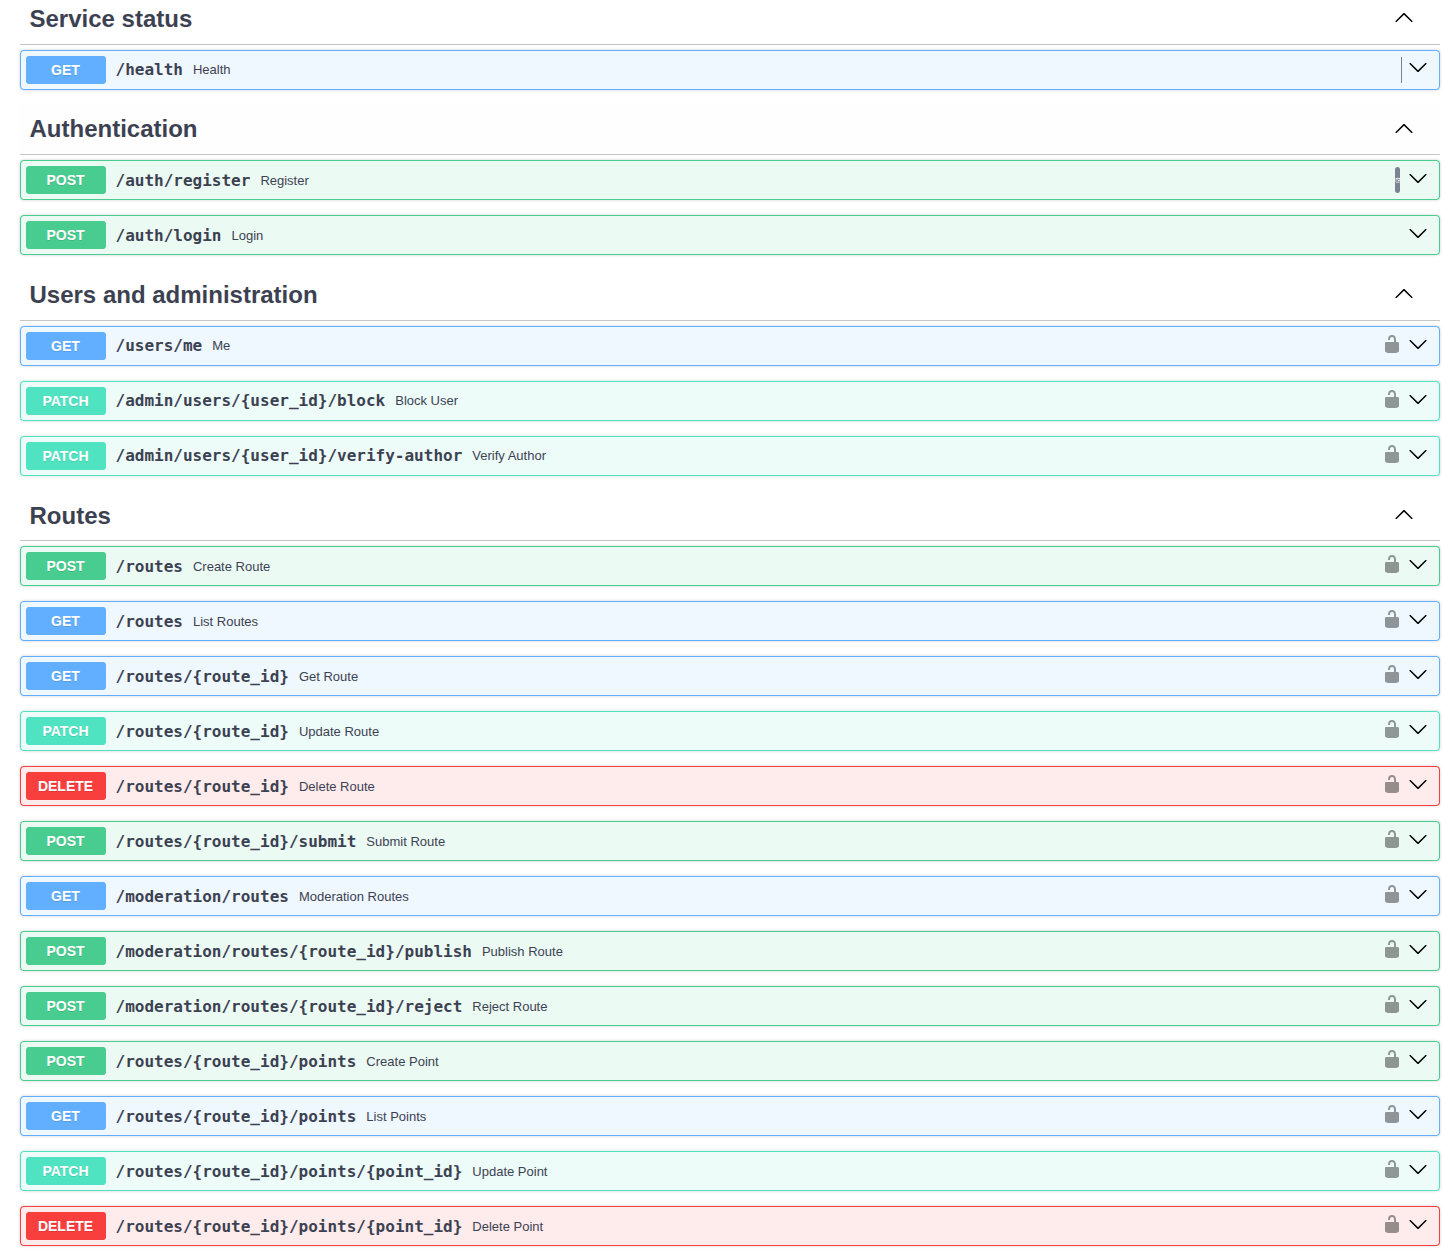
\includegraphics[width=0.95\textwidth]{service_status_authentication_users_and_administration_routes_screenshot_routes.png}
	\caption{Фрагмент Swagger-документации с группами endpoint и методами домена маршрутов}
	\label{fig:swagger-routes}
\end{figure}

\begin{figure}[htbp]
	\centering
	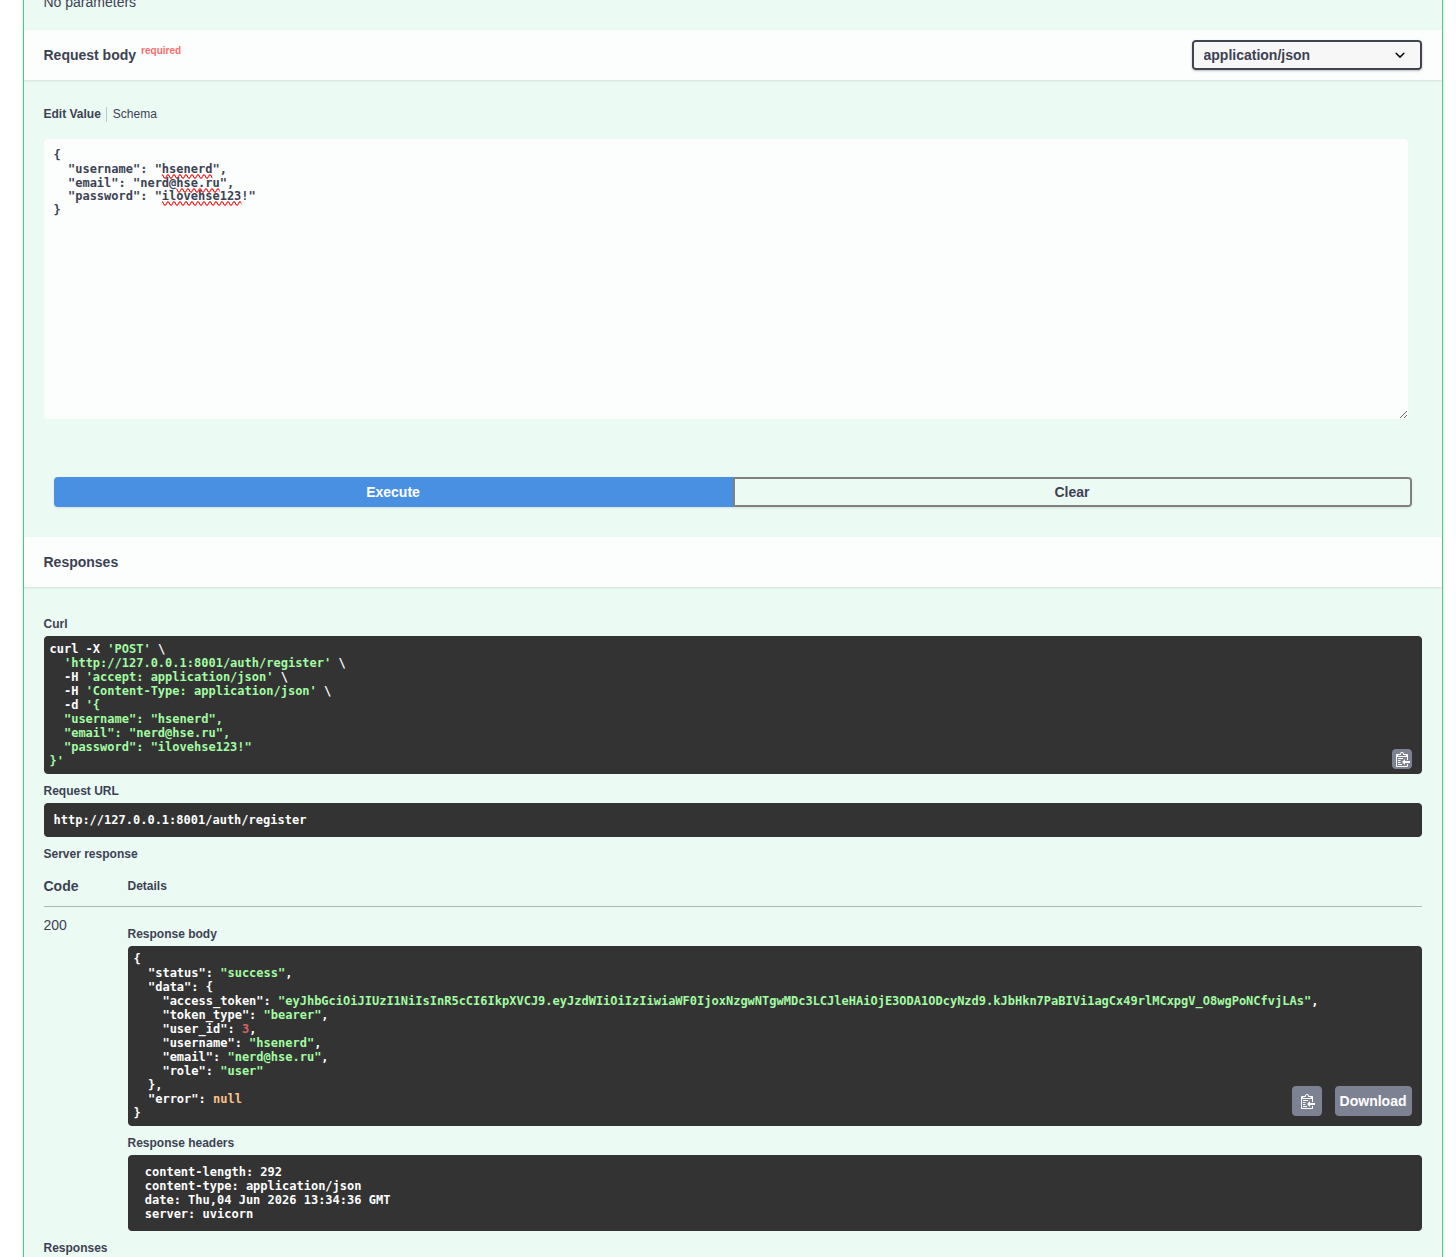
\includegraphics[width=0.95\textwidth]{successregistration.png}
	\caption{Успешная регистрация пользователя через метод \texttt{POST /auth/register}}
	\label{fig:registration-success}
\end{figure}

\begin{figure}[htbp]
	\centering
	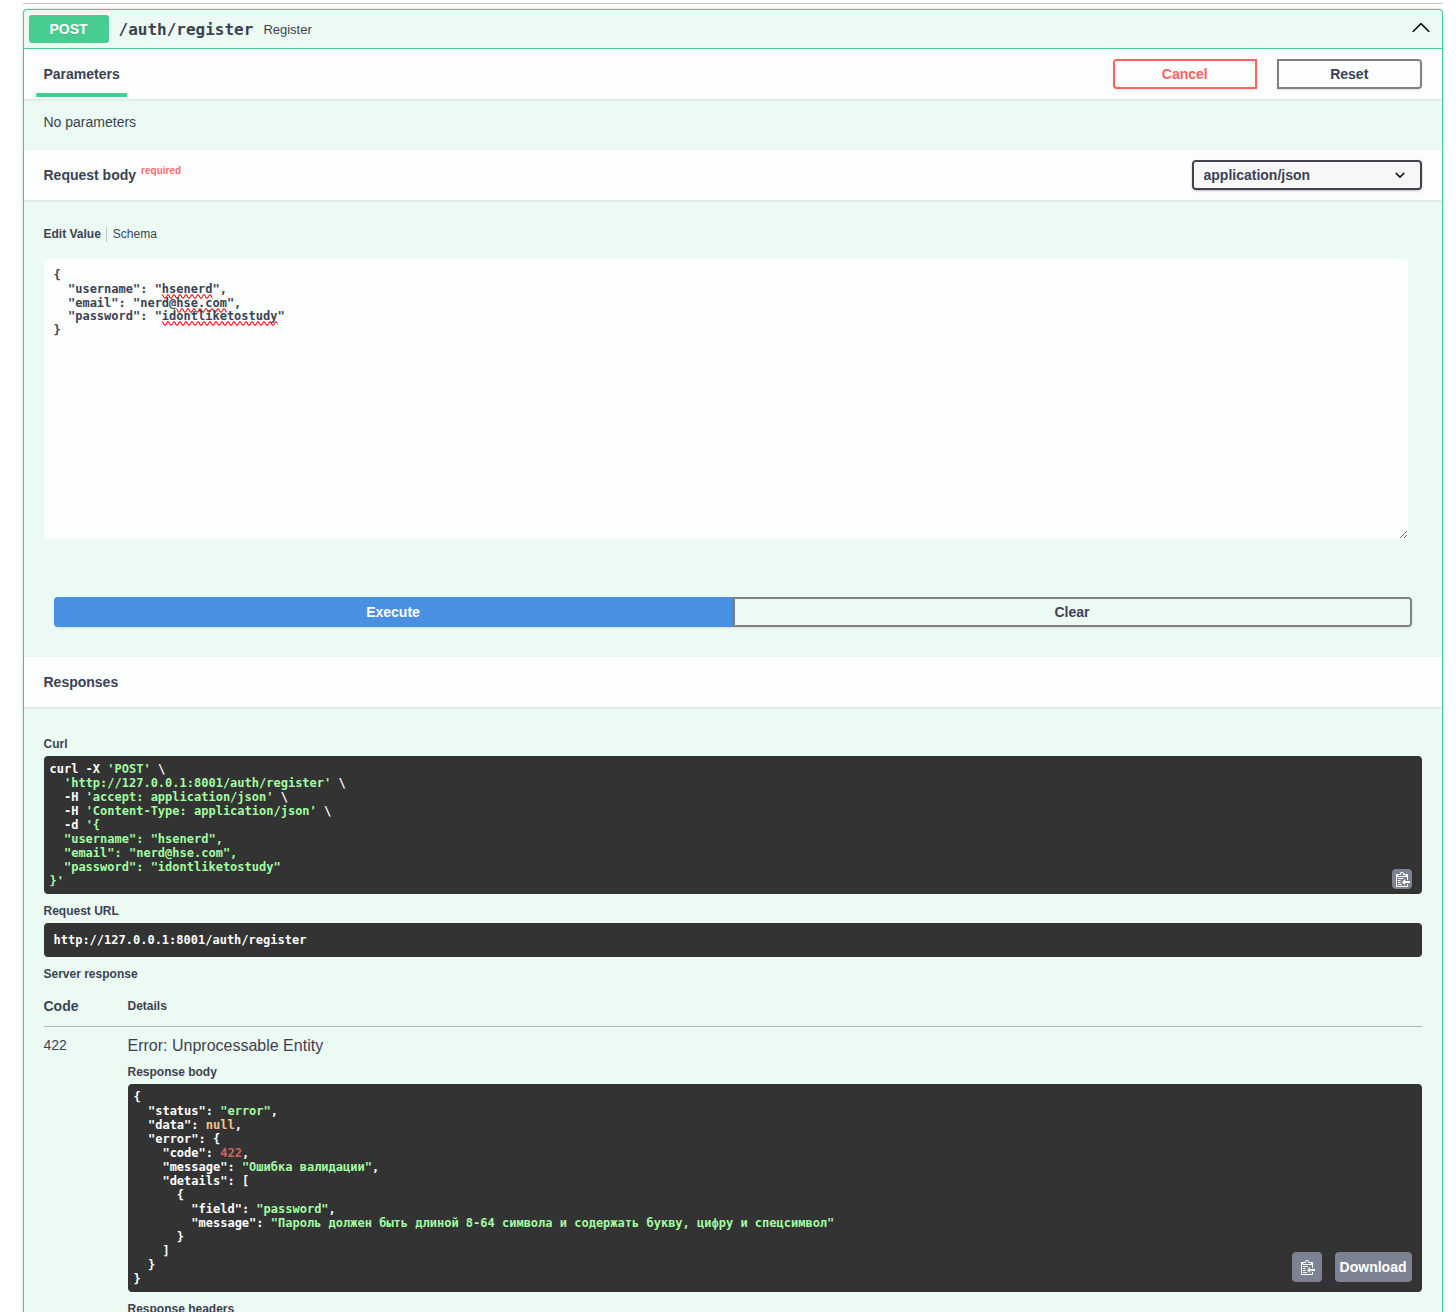
\includegraphics[width=0.95\textwidth]{errorregistration.png}
	\caption{Проверка ошибки валидации при некорректном пароле в методе \texttt{POST /auth/register}}
	\label{fig:registration-error}
\end{figure}

\clearpage

\section{Рефлексия проделанной работы}

Изначальное техническое задание оказалось достаточно широким: оно включало не только CRUD-операции, но и роли, модерацию, витрину, покупки, realtime-прогресс, аналитику, BFF и интеграции. На практике самым важным решением стало разделение проекта по доменам. Без этого логика маршрутов, впечатлений, покупок и прогресса быстро смешалась бы в одном модуле.

При реализации пришлось уточнить границы MVP. Реальные платёжные системы, полноценные ML-рекомендации и сложная мультимедийная платформа были исключены из проекта, потому что они существенно увеличивали бы объём работы, но не являлись необходимыми для демонстрации основной backend-логики. Вместо этого была реализована pay-заглушка, rule-based рекомендации и прокси/локальная заглушка для поиска мест.

Сроки разработки в целом соответствовали выбранному MVP, но часть времени ушла не на написание endpoint, а на согласование инвариантов: какие статусы допустимы, кто может видеть черновики, когда маршрут можно редактировать, какие сценарии должны завершаться конфликтом. Это нормальная особенность backend-проектов: значительная часть сложности находится не в синтаксисе API, а в правилах предметной области.

\section{Заключение}

В ходе курсового проекта был разработан backend-сервис для трэвел-приложения с маршрутами и впечатлениями. Реализация покрывает основные требования технического задания: регистрацию и авторизацию пользователей, роли, маршруты, точки маршрута, впечатления, модерацию, витрину, покупки, отзывы, рекомендации, realtime-прогресс, аналитику, BFF-методы и интеграционный endpoint поиска мест. Сервис имеет единый API-контракт, реляционную модель данных, проверку прав доступа и автоматические интеграционные тесты. Полученный прототип можно использовать как основу для дальнейшей разработки frontend, подключения реальных платёжных систем, внешних картографических API и более сложных рекомендательных механизмов.

\section{Использование инструментов искусственного интеллекта}

При подготовке отчёта инструменты искусственного интеллекта использовались только как вспомогательное средство для оформления документа: приведения текста к единому стилю, подготовки LaTeX-разметки, настройки списков, таблиц, блоков кода и структуры разделов. Содержательные решения по предметной области, техническому заданию, архитектуре backend-сервиса, реализованным функциям и выводам работы не формировались искусственным интеллектом.

Техническое задание, описание реализованного программного продукта и результаты проверки качества отражают фактическое содержание проекта. Обращение к искусственному интеллекту было строго ограничено рамками, заданными научным руководителем. Использование ИИ не заменяло самостоятельную разработку программного обеспечения, анализ требований и проверку соответствия реализации заявленным сценариям.

\newpage
\appendix

\section{Структура реализованных API-доменов}

\begin{longtable}{L{0.24\textwidth}L{0.66\textwidth}}
	\caption{Соответствие API-модулей доменам системы}
	\label{table:api-modules}\\
	\toprule
	Модуль & Ответственность \\
	\midrule
	\endfirsthead
	\toprule
	Модуль & Ответственность \\
	\midrule
	\endhead
	\texttt{auth.py} & Регистрация и вход пользователя. \\
	\texttt{users.py} & Получение профиля, блокировка пользователя, назначение роли автора. \\
	\texttt{routes.py} & CRUD маршрутов, отправка на публикацию, модерация, CRUD точек маршрута. \\
	\texttt{impressions.py} & CRUD впечатлений, публикация, отклонение, архивирование, доменный просмотр. \\
	\texttt{showcase.py} & Публичная витрина опубликованных впечатлений. \\
	\texttt{purchases.py} & Создание покупки, оплата через заглушку, список покупок пользователя. \\
	\texttt{reviews.py} & Создание и просмотр отзывов. \\
	\texttt{recommendations.py} & Rule-based рекомендации по городу. \\
	\texttt{progress.py} & Получение прогресса и WebSocket-прохождение впечатления. \\
	\texttt{analytics.py} & Список событий и агрегированная аналитика. \\
	\texttt{bff.py} & Укрупнённые ответы для экранов frontend. \\
	\texttt{places.py} & Поиск мест через внешний API или локальную заглушку. \\
	\bottomrule
\end{longtable}

\end{document}
